% !TEX root = ../main.tex
\chapter{基于深度哈希的大规模车辆重识别}
车辆重识别是现代智能交通系统中非常普遍的技术。在监控系统中, 车辆重识别可以用于对目标车辆进行自动化的监管, 定位, 以及在犯罪行为发生后进行的刑侦调查。传统的的重识别方法一般是通过将车辆照片映射到实值的特征向量并且通过欧式距离的计算将数据库中的照片根据距离进行排序来进行。然而, 尽管这样的方法可以取得较高的检索准确率, 这些高维的特征向量并不是为了快速索引匹配而设计的, 而且需要占用较大的内存空间, 同时欧式距离的计算也需要较大的计算量。 因此, 这样的方法并不适用于大规模的车辆重识别的场景中。 \par
为了解决这个难题, 本章提出了一个新型的车辆检索的框架 \textbf{DVHN}, 这是第一个将深度哈希学习引用到车辆重识别任务上的工作。 ~\textbf{DVHN}可以极大的降低内存开销并且提高检索的效率同时不会损失较多的准确度。具体来说, ~\textbf{DVHN} 通过联合的特征训练和哈希码生成训练, 使用深度卷积神经网络直接对每张图片学习一个紧凑的二进制编码。为了实现这一目的, 我们直接量化深度网络的输出, 生成离散的哈希编码, 并且增加限制条件使得哈希编码对于分类任务是最优的。 为了优化这个离散的哈希框架, 我们提出了一个交叉优化方法来同时优化离散哈希模块以及特征提取的深度神经网络。本章在两个标准的大规模车辆重识别数据集\textbf{VehicleID}和\textbf{VeRi}上进行了广泛的测试. 实验结果表明, 本章提出的算法\textbf{DVHN}在所有哈希长度上均远超当前最先进的方法。~\textbf{DVHN} 在哈希长度为 $2048$ 时可以在\textbf{VehicleID}(800)取得 $13.94 \%$ 和 $10.21 \%$的~\textbf{mAP} 和$Rank-1$ 精度提升。 在 \textbf{VeRi}数据集上, ~\textbf{DVHN} 可以在$Rank-1$上取得 $35.45 \%$的精度提升, 在~\textbf{mAP}上取得$32.72 \%$的性能提升。
\section{引言}
车辆重识别 (Vehicle Re-identification, Vehicle ReID)~\cite{liu2016deep, liu2017beyond, yan2017exploiting, guo2018learning, lou2019embedding, meng2020parsing} 由于其在智能交通系统, 智能安防领域, 以及在智能城市管理领域的广泛应用, 获得了计算机视觉研究人员的大量关注。\textbf{Vehicle-ReID}旨在给定一张查询的车辆照片, 在由不同监控摄像头拍摄的车辆照片组成的大规模车辆图片数据库中精确的找到属于同一辆车的其他照片。 一般的车辆重识别框架包含两个模块: ``特征学习模块'' 和 ``度量学习模块''。 (1)特征学习: 通过传统基于手工或者基于深度卷积神经网络的方法从车辆图片中提取有判别性的特征。 (2)度量学习: 使得上一步骤学习到的特征向量在低维空间可以保留原始图片的语义信息~\cite{chu2019vehicle}。也就是说, 语义不一致的图片在特征空间的距离尽量疏远, 而语义相近的图片应该尽量有接近的特征向量。 以往的车辆重识别方法已经在多种研究数据集上取得了令人瞩目的性能, 并且被工业界应用在一些现实任务中。 然而, 这些传统的车辆重识别方法并不能在现实生活中的大规模检索任务中进行应用。在大规模图像检索中, 被检索的图像中一般包含了数百万甚至上千万的图片数据。传统的车辆重识别方法一般有下面的劣势, 限制了其在大规模场景的应用。 首先, 在数据库中包含超大量的图片时候, 高维的实值特征向量的存储开销变得极其大。例如, 存储一个 $2048$维的浮点$64$类型的特征向量需要占据 $16$ 千字节(Kilobyte, KB)。对于一个数据库中具有1千万张图片的检索任务而言, 总共需要的内存高达 $150$ 吉字节 (Gigabyte, GB)。 除开内存开销, 检索时需要使用查询的特征向量与数据库中所有的存储的特征向量进行欧式距离的计算。然而, 欧式距离的计算耗时大~\cite{lin2015deep}, 也使得这种方法无法被应用在对检索速度要求较高的任务中。\par
近年来, 由于其低内存开销以及高检索效率, 深度哈希学习已经被广泛应用在通用的图片检索任务中。深度哈希的目标是通过学习一个哈希函数将图片映射到一个低维的汉明空间, 同时在汉明空间里保留其在原始图片的语义相似性~\cite{lin2015deep, cakir2019hashing, cao2016correlation, cao2017hashnet}。因为一个 $2048$位的汉明哈希码仅仅只需要占据 $256$ 字节的内存, 对于上面所述的1亿张图片的数据库只需要不到 $2.4$ GB的内存开销, 相比较基于实值的特征向量而言, 节省了 $147$ GB 的内存开销。另外, 如文章~\cite{ong2016improved}所述, 二进制汉明哈希码之间的汉明距离可以通过 CPU硬件指令 \textit{XOR} 进行加速。 通常来说, 汉明距离的计算可以使用几个机器指令来完成, 相比较欧式距离的计算来说, 极大的降低了计算的时间开销。 \par
被上述的深度哈希的优势所启发, 本章思考了将深度哈希算法直接引入到车辆重识别问题, 来完成大规模车辆重识别任务的可能性。尽管深度哈希在通用图片检索取得了较好的性能表现, 由于车辆重识别任务的独特性和难度, 直接应用这些深度哈希的算法并不能取得可以令人接受的性能表现。车辆重识别受光照变化, 背景繁杂, 遮挡, 以及不同拍照视角的影响导致了问题的困难性。传统的深度哈希方法很难学习到强健的有判别性的特征表示。例如, 一个经典的深度哈希方法~\textbf{SFH}~\cite{lai2015simultaneous} 是第一个端到端的监督的深度哈希框架。 它采用了一个三元损失函数并且使用一个divide-and-conquer模块来生成二进制哈希码。同时在深度卷积神经网络的输出后采取L1-norm来限制网络生成二进制的编码。然而, 这些方法是被设计用在当数据库中检索图片的类别较少的场景。 而在车辆重识别场景中, 数据库中有数以千计甚至上万的车辆, 而且每辆车包含的照片受上述多方面的影响具有较大的差异。 因此, 现成的深度哈希方法只能学习到此优的图像表征, 从而只能生成次优的二进制编码。\par
本章提出了一个新型的基于深度哈希的框架-\textbf{DVHN}-用于高效的的大规模车辆重识别场景。~\textbf{DVHN}充分的吸收了深度哈希的优点但是同时也没有牺牲检索的准确度。它主要包含四个部分: (1) 与以往基于图片对或者图片三元组的传统的哈希方法不同, 本章提出一种在每个批次输入中动态生成困难三元组的方法。(2) 一个基于深度卷积神经网络的特征提取方法。(3) 一个基于度量学习的哈希码生成模块来使得生成的哈希编码可以保留原始图片的视觉相似性。(4) 一个离散汉明哈希模块。 \par
对于保持相似性的度量学习方法, 我们采取一个基于困难三元组挖掘的三元损失函数 (batch-hard triplet loss)来尽量拉近视觉相似的图片在特征空间的距离, 相反, 推远视觉不相似的图片在特征空间的距离。另外, 为了使哈希码多保存具有判别性的行人特征, 本章另外加入了一个身份损失, 实际上是一个基于交叉熵的分类损失函数, 将每一个行人视作一个不同的类别。 对于离散汉明哈希模块, 我们直接使用不能导的 \textit{sign} 函数将神经网络的输出直接量化成离散的二进制编码, 并且限制这些学习到的二进制编码是对于分类最优的。 因为 \textit{sign} 函数不可导, 无法通过反向传播进行端到端的训练, 我们设计了一个新型的交叉优化方法来对~\textbf{DVHN}进行优化。在测试阶段, 对于所有查询图片以及数据库中的图片, 我们将它们编码成二进制的哈希码,然后将所有的数据库中的图片通过其与查询图片的哈希码的汉明距离进行从小到大的排序。 \par
本章主要做出如下的贡献:
\begin{enumerate}
    \item 本章分析了阻碍现有的车辆重识别的算法在大规模现实场景应用的主要障碍。我们进行了最初期的使用深度哈希学习来进行大规模车辆重识别的尝试。
    \item 本章提出了一个新型的框架, 以一种端到端的方式对车辆图片学习紧凑的哈希编码。本章提出一个新型的离散汉明哈希模块来学习二进制哈希编码, 同时保证哈希编码在分类任务上是最优解。为了解决困难的离散优化的问题, 我们采取一种交叉优化的方法, 通过离散编码学习到二进制哈希码后, 通过二进制哈希码以及度量学习的损失函数来监督训练神经网络进行表征学习。
    \item 本章基于Pytorch实现了多个先进的深度哈希算法, 并且仔细完备的训练并且测试了它们在标准的车辆重识别数据集上的性能。本章从头训练了72个模型, 对这一方向的研究提供了宝贵的基础数据。通过全面的测试以及比较, 我们证实了本章提出的\textbf{DVHN}算法的有效性, 并且证实了本章的相比较现有的先进算法可以获得极高的性能增长。
\end{enumerate}

\section{相关工作}
在这一小节, 我们主要阐述先前的与本章提出的算法相关的工作。我们主要根据它们是否采用了二进制特征向量来将它们分为两个类别: ``基于哈希的图像检索'' 和 ``车辆重识别''。
\subsection{基于哈希的内容检索}
近年来基于哈希的大规模内容检索已经获得了工业界和学术界的广泛关注~\cite{indyk1997locality, weiss2008spectral, gong2012iterative} \cite{heo2012spherical, jegou2010product, ge2013optimized, li2018deep}。根据它们提取特征的方法, 现有的哈希方法主要可以分为两个类别: 浅哈希方法和基于深度学习哈希方法。\par
典型的浅哈希方法通常是基于手工特征来学习哈希编码。一个经典的这方面的算法是局部敏感性哈希 LSH~\cite{indyk1997locality}, 其通过寻找一个局部敏感的哈希族来进行哈希编码的生成。这种哈希族内的哈希函数对于相似的对象生成的哈希码会有碰撞的概率远大与不相似的对象。随后, 基于 LSH, Charikar等人提出 SIMHASH~\cite{charikar2002similarity} 通过结合取整方法实现一系列的保距哈希函数。尽管基于 LSH 的方法取得了不错的性能, 但是它们需要比较长的哈希编码才能取得较好的性能结果。 2008年, Weiss 等人~\cite{weiss2008spectral} 提出了通过最小化图像对的带权的汉明距离来生成哈希编码。尽管这些基于手工特征的哈希方法取得了一定程度上的成功, 但是当被应用到具有较大的类内变化(Intra-class Variation)的现实数据中时, 由于基于手工的特征提取方法无法精确的保存图片中具有判别力的部分, 这些方法只能取得较低的性能表现。\par
考虑到这一点, 基于深度学习的哈希方法开始涌现~\cite{cao2017hashnet, fan2020deep, li2015feature, zhu2016deep, liu2016deep}。根据这些方法是否会使用到人工标注的标签进行监督训练, 基于深度学习的哈希方法也可以分为: 有监督的哈希方法和无监督的哈希方法。无监督的哈希方法通过探索数据内部自带的特征信息来生成二进制码。经典的例子有~\cite{song2018binary, yang2019distillhash, tu2020mls3rduh, qiu2021unsupervised, luo2020cimon}。具体来说, Song等人~\cite{song2018binary} 提出一个二进制的生成对抗网络来通过一种无监督的方式将图片嵌入成二进制码。具体来说, 通过Generator在encoder生成的二进制码上进行条件生成原图片, 通过Discriminator进行判别生成的原图片的优劣, 可以促使Encoder生成的二进制哈希码保存更多原始图片中的信息。Yang 等人提出了 DistillHash~\cite{yang2019distillhash}, 在原始数据集上生成一个提炼的新的包含很多数据对的数据集, 每个数据对被认为是来自同一个类别, 也就充当了监督训练的标签。 Tu 随后提出 MLS3RDUH~\cite{tu2020mls3rduh}  引入一个机制通过探索特征内在的流型结构来通过数据的余弦相似度重建局部的语义相似度。 Qiu ~\cite{qiu2021unsupervised}提出通过采用带有信息瓶颈的对比学习来进行无监督的哈希学习。随后, Luo 等人提出 Cimon~\cite{luo2020cimon}通过全局的优化以及相似性的统计分布来得到可靠并且光滑的指导。本章的工作属于带监督的哈希范畴, 通过人工标注的标签提供监督信号。2014年, Xia~\cite{xia2014supervised} 提出第一个基于深度学习的监督哈希框架。它提出一种两阶段哈希的方法先将相似度矩阵$S$ 分解成汉明矩阵$H$ 和 $H^T$的乘积, 其中 $H$的每一行代表一个训练图片数据的哈希编码。然后, 在下一阶段, 卷积神经网络通过第一阶段得到的哈希码作为监督信号来进行监督训练。随后, Lai等人提出一个端到端的深度哈希框架~\cite{lai2015simultaneous}, 通过三元损失函数以及一个divide-and-encode 模块来端到端的学习图像特征以及生成二进制的哈希编码。Zhu 随后提出 DHN~\cite{zhu2016deep} 基于贝叶斯学习框架设计一个基于成对训练数据的损失函数来进行相似度保留的哈希码生成。Cao 随后提出 DCH~\cite{cao2018deep} 通过使用一个柯西分布 (Cauchy Distribution) 来替换DHN框架中使用Sigmoid函数来度量两张图片输出的相似概率。Wu 提出了一个增量哈希框架 (incremental hash)~\cite{wu2019deep}, 这个框架不需要每次当数据库中的图片数量增加的时候重新训练模型, 更加具有现实可用性。 Fan 随后提出 DPN~\cite{fan2020deep} 通过一个深度极化损失(Polarized Loss)来监督模型进行二进制哈希码的生成, 使得不再需要加入常用的量化损失函数来控制模型的输出和量化后的二进制码的误差。尽管相比较无监督的方法, 基于监督的深度哈希取得了更加优越的性能表现, 这些方法并不是为了大规模车辆重识别而设计, 没有考虑到车辆重识别任务具有的特殊的挑战, 在Vehicle ReID任务上只能取得一般的性能表现。 \par
\subsection{基于深度学习的车辆重识别}
由于车辆重识别在数字监控, 智能交通~\cite{zhang2011data}, 城市计算~\cite{zheng2014urban}等领域的大规模应用, 基于深度学习的车辆重识别\cite{liu2016large, liu2016deep, wang2017orientation} \cite{liu2017provid, bai2020disentangled, meng2020parsing}在这些年开始受到工业界和学术界的大规模的关注~。车辆重识别由于其较大的类内差异(Intra-class variation)和较小的类间差异(Inter-class variation)而非常具有挑战性, 这是由于不同的车属于同一品牌或者统一模具生产而外观非常相似。一部分的工作聚焦在提高学习到的特征表示的辨别力上。 Liu~\cite{liu2017beyond} 提出一个双流的神经网络来将不同模态的车辆照片映射到可以比较的欧式空间。Yan~\cite{yan2017exploiting} 提出通过探索多粒度的排序限制来学习特征。随后, Guo 等人提出通过一种从粗粒度到细粒度的学习方法来学习更加强健的特征表示。2019年, He~\cite{he2019part} 采取了提取车辆的局部分块的表征来帮助全局的特征训练。Lou ~\cite{lou2019embedding}设计了一个端到端的就对抗学习的网络来学习有判别性的特征。
Zheng ~\cite{zheng2020vehiclenet} 提出了另一个大规模车辆重识别的数据集 \textbf{VehicleNet}并且设计了一个两阶段学习框架来进行检索训练。Jiang~\cite{jiang2021robust}提出通过一个基于分块学习以及将车辆的刚性结构先验信息加入神经网络来学习强健的特征表示。 2022年, Li~\cite{li2022super} 提出了一个基于超分的车辆模块协同网络 (SPCN)来进行车辆重识别。 \par
另一部分的车辆重识别工作主要关注学习对视角不变 (Viewpoint Invariant)的特征~\cite{wang2017orientation, zhou2018aware, tang2019pamtri, bai2020disentangled}。2017年, wang提出通过定义多个关键部位, 对关键的部位进行局部特征抽取而得到对朝向不变的特征表示。同时提出一种在空间和时间维度上的标准化策略来提高检索的准确性。Zhou 随后提出一种新的机制~\cite{zhou2018aware}通过单个视角的信息生成多视角的特征。 Zhou 提出一种对于车辆摆放信息感知的多任务学习算法来学习对于视角不变的特征。Bai ~\cite{bai2020disentangled}随后提出可以将特征解耦成对于朝向特有的(Oritentation-specific)以及朝向恒定的(Orientation-invariant)的特征来进行重识别任务。Zhu ~\cite{zhu2019vehicle}提出基于四元组的损失函数来进行特征抽取以及度量学习而 Chen 等人~\cite{chen2020vehicle}则提出了一种端到端的基于距离的深度神经网络, 它可以学会区分车辆的局部和全局的不同性来进行重识别。Liu 提出一种车辆解析方法来学习有判别度的车辆局部信息以及建造了一个分块的邻接图来对每个不同部分的特征的关联进行建模。为了减轻剧烈的外表变化带来的影响, Jin 随后设计了一个新型的多中心度量学习的框架来对车辆外观的隐藏的观察点进行建模而不需要额外的监督标签。尽管这些方法取得了一些成果, 以上提及的车辆重识别方法都是基于实值的特征向量并且依赖于欧式距离的计算来对数据库中的图片进行排序和检索。这些方法无法适用于实际现实中的大规模车辆重识别的场景, 以及对与检索速度要求较高的场景。
\section{基于深度哈希的重识别算法}
\subsection{本章主要符号定义以及问题定义}
在本章中, 我们使用书法大写字母 (Calligraphic Uppercase), 例如 $\mathcal{F}$ 来表示映射函数。我们使用粗体大写字母 (Bold-face Uppercase) 如 $\mathbf{B}$ 来代表集合. 粗体小写字母如 $\mathbf{b}$在全章中代表向量。我们使用斜大写字母 (Italic Uppercase)来代表图片, 如 $\textit{I}$。 同时, 在全章中, sign激活函数直接由 $\textit{sign}$ 来表示。\par
\textbf{问题定义:} 假设 $\mathbf{X} = \{\textit{I}_i\}^N_{i=1}$ 是一个包含了$N$个训练数据的车辆检索训练数据集。 $\mathbf{Q} = \{I_i^q\}^{N_{q}}_{i=1}$ 和 $\mathbf{G} = \{I^g_i\}^{N_{g}}_{i=1}$是对应的查询集和被检索的数据库图片集。$\mathbf{Y} = \{\textit{y}_i\}^N_{i=1} \in \{0,1\}^C$是对应的标签集, 其中$C$是对应的车辆数。 基于深度哈希的车辆重识别的目标是学一个非线性的哈希函数 $\mathcal{H}: I \mapsto \mathbf{b} \in \{0,1\}^K $, 通过输入一张图片$\it{I}$并且将其映射成一个 K 位的二进制哈希向量 
$\mathbf{f}$。

同时需要保证每张车辆照片经过映射后的哈希向量需要保存原车辆照片的视觉相似性。整个基于学习的哈希函数可以由如下公式表示:
\begin{equation*}
    \mathbf{b}  = \mathcal{H}(I) = \mathbf{\it{sign}} (\mathcal{F}_{hash}(\textit{I})) 
\end{equation*}
其中 $\mathcal{F}_{hash}$ 代表生成哈希向量的非线性的深度神经网络, $\it{I}$是输入的车辆照片。 $\mathbf{\it{sign}(v)}$是一个符号函数, 它输出 $1$ 如果 $v \geq 0$, 反之输出$-1$。
本章提出一个新型的针对车辆重识别设计的哈希框架~\textbf{DVHN}。在接下来的小节中, 我们会着重详细的介绍模型的实现细节。我们先简单的介绍了我们的基础神经网络架构。随后, 我们介绍用于进行相似度学习的度量方法。之后, 我们详细的阐述了离散哈希学习的方法。接着, 我们介绍了采用的优化整个架构的交叉优化方法。最后, 我们简单的介绍了训练和测试的检索过程。
\begin{figure}[!htp]
    \centering
    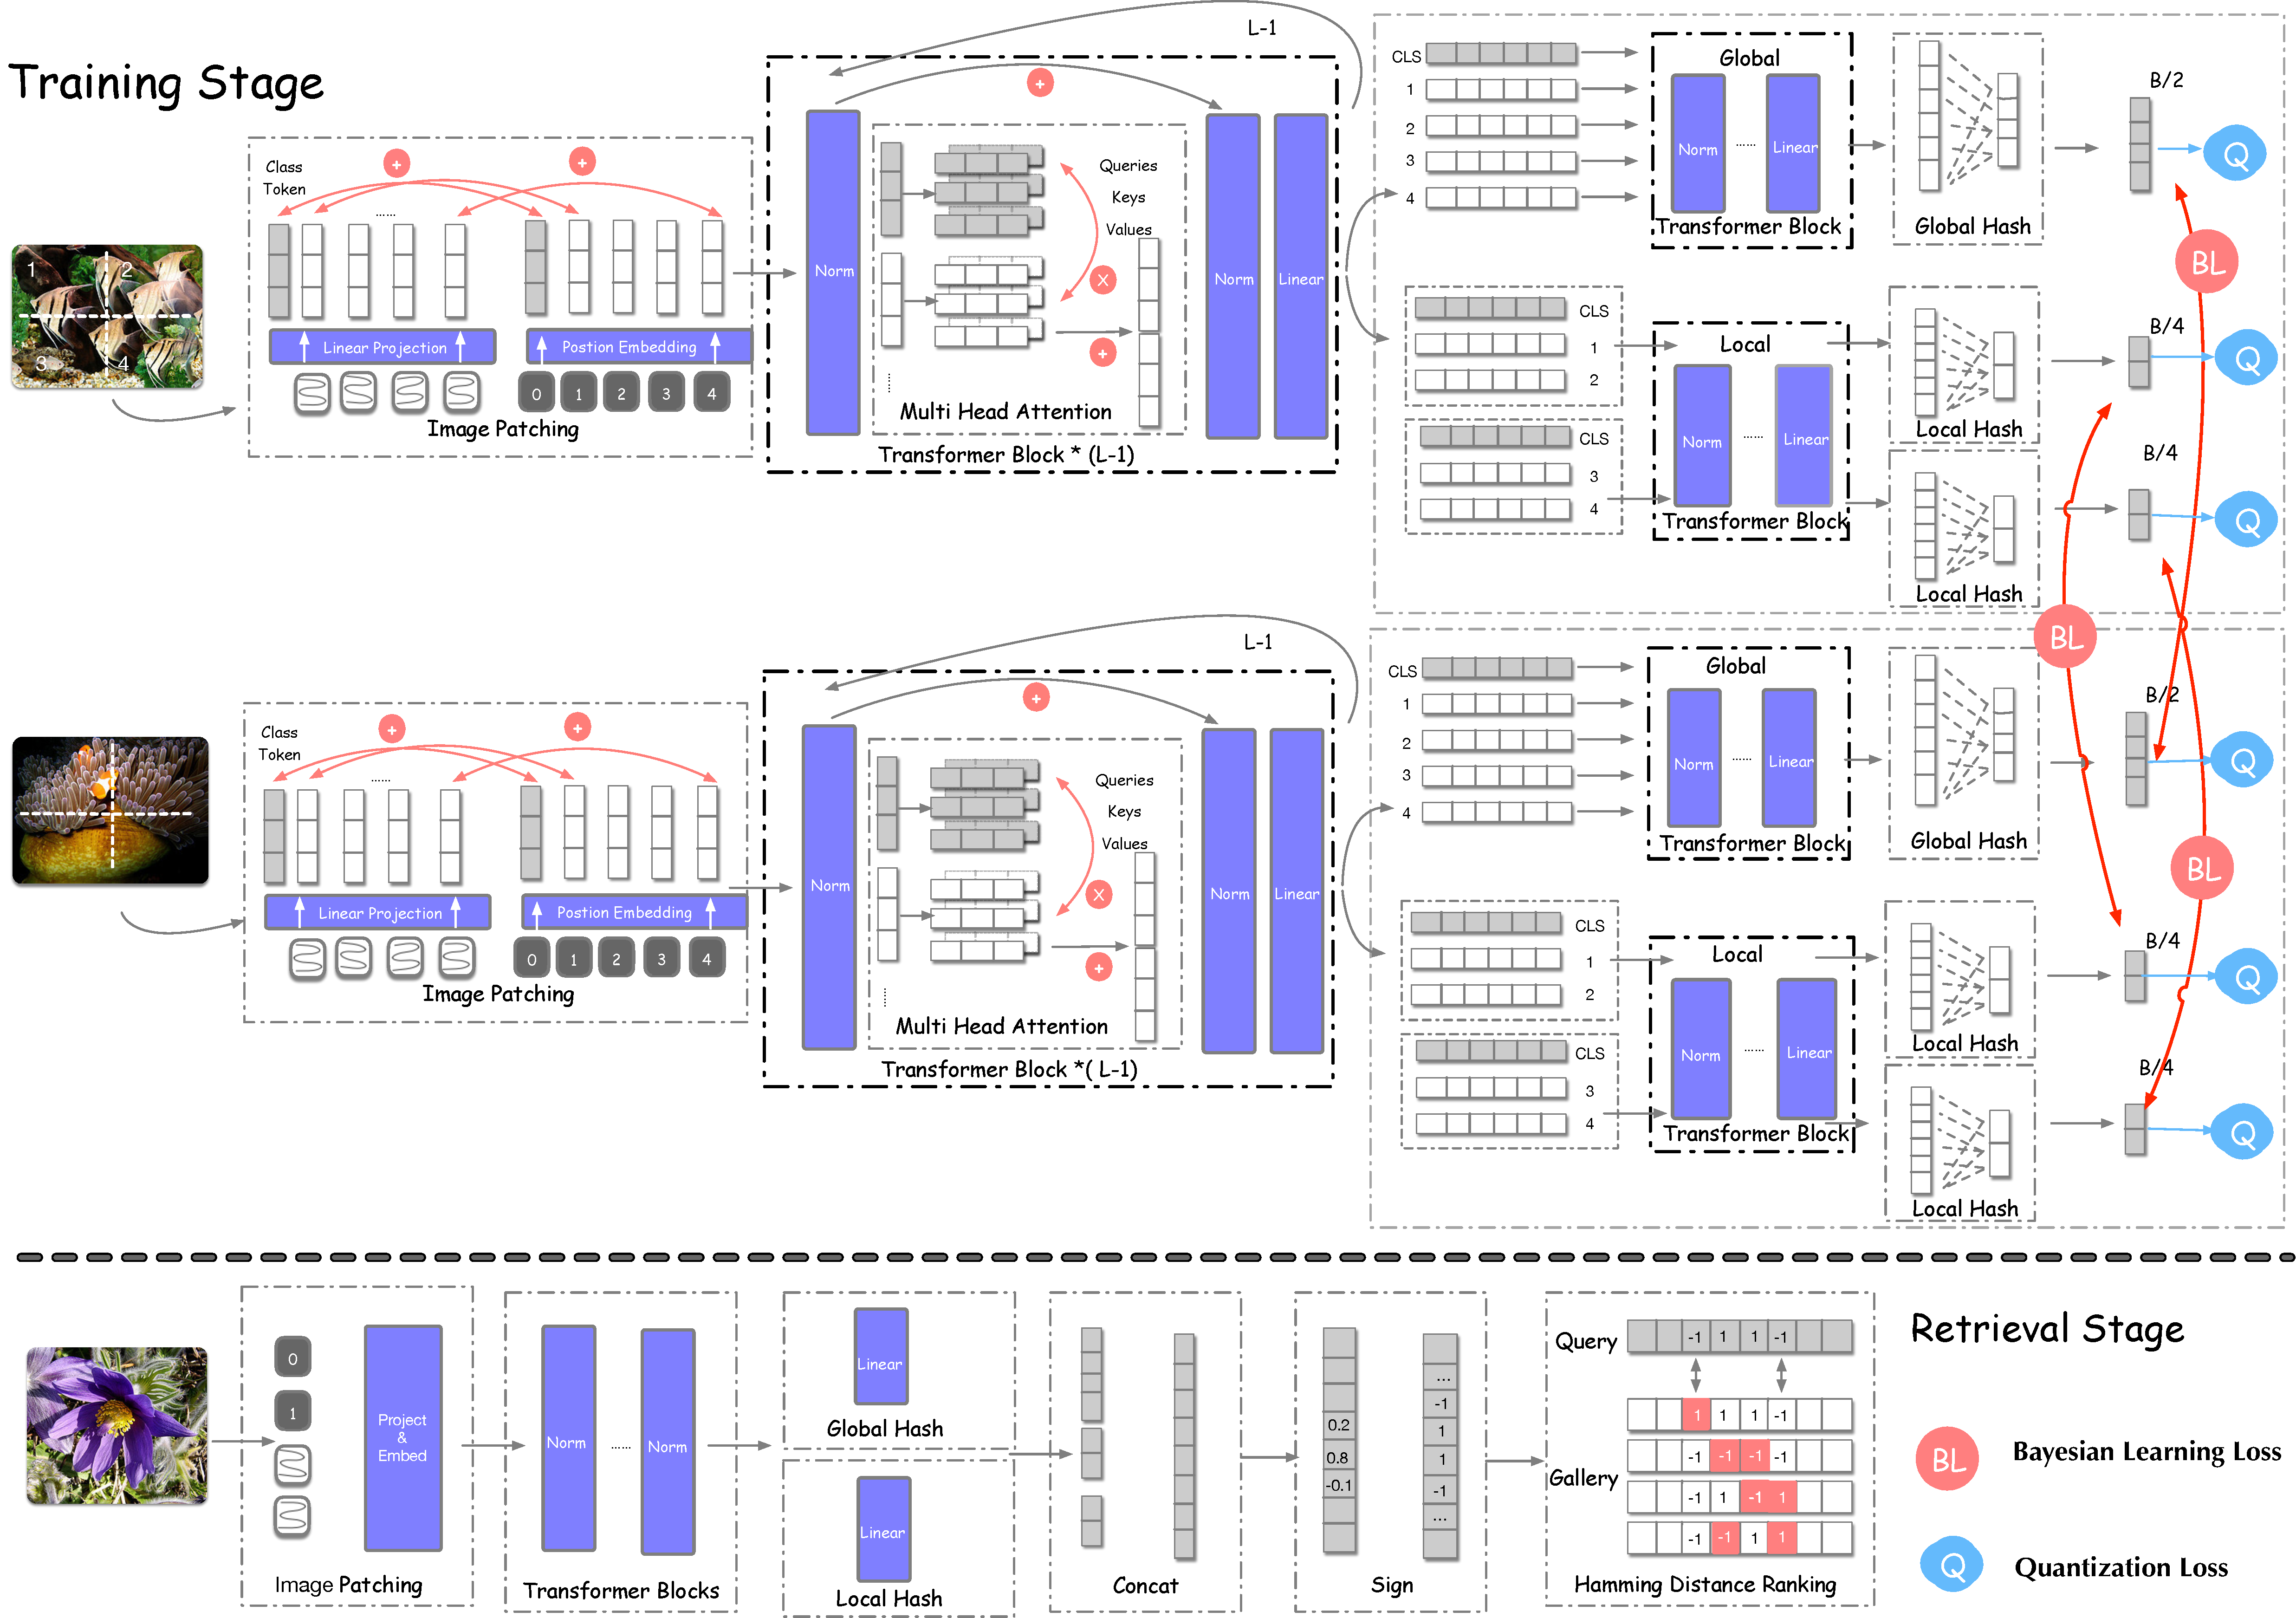
\includegraphics[width=15cm]{03/architecture.pdf} \\
    \bicaption[基于深度哈希的大规模车辆重识别框架]
      {基于深度哈希的大规模车辆重识别框架图,包含两个阶段。上图阐述神经网络学习生成有效的哈希编码的过程, 包含一个身份损失和一个基于困难组的三元损失函数以及离散哈希模块。下图阐述了测试过程。在测试阶段, 检索和数据库图片都被编码成二进制编码, 然后通过与检索的图片的汉明距离进行排序。}
      {The framework of DVHN. It basically contains two stages. The top part illustrates the process of learning to produce effective hash codes. The
      bottom demonstrates the testing process. During testing, the query and gallery images are encoded into binary discrete hash codes with the trained model.
      Then, the gallery images are ranked by computing their Hamming distances to the query image.}
   \label{fig:archvehicle}
\end{figure} 
\subsection{用于生成哈希向量的网络}
我们采取 \textbf{ResNet-50}~\cite{he2016deep} 作为基础的特征提取神经网络, 用$\mathcal{F}_{\theta}$表示。图片$\it{I}_i$丛$\mathcal{F}_{\theta}$输出的特征向量$\mathbf{f}_i$的过程如下所示:
\begin{equation}
    \mathbf{f}_i = \mathcal{F}_{\theta}(I_i)
\end{equation}
为了生成有不同长度的哈希码, 我们基于主干网络设计了一个额外的哈希层。具体来说, 在全局平均池化层(Global Average Pooling)后, 我们增加了一个全连接层, 它接收$M$维度的特征向量 $\mathbf{f}$ 输出 $K$维度的连续的哈希向量:
\begin{equation}
    \mathbf{h} = \mathcal{F}_{\theta_1}(\mathbf{f}) = \mathbf{f}W_1^T + \textbf{b}
\end{equation}
其中$W_1 \in \mathbb{R}^{M\times K}$ 和 $\mathbf{b} \in \mathbb{R}^{K}$ 代表全连接哈希层的权重以及偏差参数。 而$K$是代表汉明哈希码的长度。值得注意的是, 不像之前的深度哈希方法采取 \textit{tanh} 或者 \textit{sigmoid} 函数来将神经网络的输出强制接近二进制输出, 我们采取一个量化损失函数 $quantization loss$ 来使得神经网络的输出接近二值, 具体细节会在接下来的小节中详细阐述。
\subsection{基于相似度保留的特征学习}
我们将输入的车辆图片组织成三元样本, 并且将哈希函数学习的问题转化为一个相似度保留的特征学习问题。具体来说, 被Hermans~\cite{hermans2017defense}的工作所启发, 我们在每次输入前, 先随机采样 $P$ 个车辆, 随后, 我们随机对于每一辆车采样$K_1$张图片来组成一个具有$P*K_1$张图片的批次输入。对于在批次中的每一张图片$\it{I}_i$, 我们会将它视为锚定图片(Anchor Image), 然后找到一张和$\it{I}_i$属于同一辆车但是距离最远的图片$\it{I}_i^+$。同样的方法,我们也会在批次中找到一个在某个距离指标$D$下最难的负样本$\it{I}_i^-$, 即和图片$\it{I}_i$属于不同的一辆车但是距离却最近的图片。 通过这样的方法, 我们可以得到一个训练数据集 $\mathbf{T_{1}} = \{(I_i, I_i^+, I_i^-)\}_{i=1}^{P*K_1}$。对于每一张图片 $I$, 对应的连续的哈希向量 $\mathbf{h}$ 可以通过以下公式得到:
\begin{equation}
    \mathbf{h}_i = \mathcal{H}(I_i) = \mathcal{F}_{\theta_1}(\mathcal{F}_{\theta}(I_i))
\end{equation}
其中 $\mathbf{h}_i$是$\it{I}_i$对应的哈希向量。 $\mathcal{F}_{\theta}$代表主干非线性的卷积神经网络,而$\mathcal{F}_{theta_1}$则代表基于全连接神经网络的哈希层。因为我们的目标是需要保存图片在汉明空间的相似性, 我们提出了以下的限制:
\begin{equation}
    \mathcal{D}_H(\mathbf{h}_i, \mathbf{h}_i^+) < \mathcal{D}_H(\mathbf{h}_i, \mathbf{h}_i^-) 
\end{equation}
其中, $\mathcal{D}_H$代表了汉明距离。这个公式表明, 我们希望anchor图片和其最难的正样本$\it{I}_i^+$的汉明距离应该要小于和对应的最难负样本的距离。我们可以观察到汉明距离与内积有以下的线性关系:
\begin{equation*}
    \mathcal{D}_H(\mathbf{h}_i,\mathbf{h}_j) = \frac{1}{2}(B - \langle \mathbf{h}_i,\mathbf{h}_j \rangle)
\end{equation*}
因此, 在本文中我们使用内积来作为汉明距离的一个替代计算方法, 以便于汉明距离的计算。\par
接下来, 我们可以用公式表示基于三元图片组的相似性保留损失函数:
\begin{equation}
    \begin{array}{l}
    \begin{aligned}
    L_{Triplet} (h)
    &= \sum_{i \in \mathbf{T_{1}}} [\alpha + \mathcal{D}_{H}(\mathbf{h}_i,\mathbf{h}_i^+) - \mathcal{D}_{H}(\mathbf{h}_i, \mathbf{h}_i^-)]  \\
    &=  \sum _{i=1}^{P} \sum _{a=1}^{K}[\alpha+\overbrace{\max _{p=1 \ldots K}\left\|e_{i}^{a}-e_{i}^{(p)}\right\|_{2}}^{\text {hardest positive}}  \\
    &- 
    \underbrace{\min _{n=1 \ldots K \atop j=1 \ldots P} \|e_{i}^{a}-e_{j}^{(n)}\|_{2} }_\textrm{hardest negative}]
    \end{aligned}
    \end{array}
    \label{eq:tripletloss}
    \end{equation}
其中 $P$代表输入批次中有的车辆总数, $K$ 代表批次中每辆车包含的图片数量。$e_{i}^a$ 代表属于车辆 $i$ 的anchor的向量。$\alpha$代表三元损失函数的边界参数。\par
为了使学习到的特征向量可以保留更多的具有判别力的特征, 我们另外在主干网络输出的特征向量$\mathbf{f}$后增加来了一个身份损失函数(Identity Loss)。为了实现这个目标, 我们另外增加了一个全连接层充当分类器。如图~\ref{fig:archvehicle}所示, 一个输出维度的$N_C$的全连接层$\mathcal{F}_{\theta_2}$被添加在$\mathbf{f}$之后, 其中$N_C$是训练数据集中的车辆数。通过将每一辆车当成分类任务中的一个类别, 我们可以将身份损失函数表示成为一个分类损失函数:
 $L_{Identity}$ as:
\begin{equation}
L_{Identity}(f)=-\sum_{i=1}^{P*K} \log \frac{e^{{W}_{y_{i}}^{T} \mathbf{f}_i }}{\sum_{k_1=1}^{N_C} e^{{W}_{k_1}^{T} \mathbf{f}_{i}}}
\label{eq:identity}
\end{equation}
其中 $W_k$是对于第$k$辆车的权重向量, $P \times K_1$是批次中所有的图片, $N_C$是输入批次中总共的车辆数。
\subsection{离散哈希学习}
离散哈希模块核心假设是学习到的二进制汉明哈希码需要保存图片的类别信息。具体来说, 对于每一张图片$\it{I}_i$, 二进制汉明码$\mathbf{b}_i$可以通过对连续的哈希向量$\mathbf{h}_i$使用 \textit{sign} 函数得到:
\begin{equation}
    \mathbf{b}_i = \textit{sign}(h_i) = \textit{sign}(\mathcal{H}(\textit{I}_i))
\end{equation}
其中 $\textit{sign}(x)$的定义如下:
\begin{equation}
\operatorname{sgn}(x)=\left\{\begin{array}{c}
1, x>=0 \\
-1, x \le 0 
\end{array}\right.
\end{equation}
我们随后采取一个简单的线性分类器利用二进制的哈希码来重建真实的标签如下所示:
\begin{equation}
    y_i = W^T_h\mathbf{b}_i
\end{equation}
其中  $y_i \in \{0,1\}^C$, $C$是车辆的数量, $W_h$是分类器的权重参数。我们可以将离散哈希损失函数写作:
\begin{equation}
    L_{Quant}(\mathbf{b}) =  \mu\sum_{i=1}^{N}\left\|y_{i}-W^{T}_h \mathbf{b}_{i}\right\|_{2}^{2}+\nu \|W_h\|_{F}^{2}  
\end{equation}
其中 $\|\cdot\|_{2}$ 是一个向量的 $l_2$ 范数 而$\|\cdot\|_{F}$ 则是一个矩阵的弗罗贝尼乌斯范数 (Frobenius Norm )。
\subsection{交叉优化算法}
我们可以将最终的损失函数写作为:
\begin{equation}
    L_{Total} = \lambda L_{Triplet}(\mathbf{h})  + \sigma L_{Identity}(\mathbf{f}) + L_{Quant}(\mathbf{b})
    \label{eq:totall}
\end{equation}
其中 $\lambda$, $\beta$ and $\sigma$为三个预先定义的系数来控制各个部分的损失函数对目标函数的影响。最直接的优化这个目标函数的想法就是直接利用标准的随机梯度下降算法来优化这个目标函数~\ref{eq:totall}。然而, \textit{sign} 函数是不可导的, 梯度无法通过这个函数进行反向传播。因此, 目标函数的第三个部分$L_{Quant}$不能像第一第二个部分的损失函数一样用随机梯度下降算法直接优化。我们将第三个部分展开为:
\begin{equation}
    \begin{aligned}
     L_{Total} &= \lambda L_{Triplet}(\mathbf{h})  + \sigma L_{Identity}(\mathbf{f})) \\
     &+\mu \sum_{i=1}^{N}\left\|y_{i}-W_h^{T} b_{i}\right\|_{2}^{2}+\nu\|W_h\|_{F}^{2} 
    \end{aligned}
       \label{eq:totalfold}
   \end{equation}
为了绕过\textit{sign}函数带来的梯度消失的问题, 之前的工作一般采取\textit{tanh}和\textit{sigmoid}函数在训练阶段来生成接近二值的连续性的输出而在测试阶段再使用\textit{sign}函数来获得二值的哈希码。然而这样的优化方法是在优化原始目标的一个放松后的目标函数, 导致优化结果会偏离原始目标从而导致次优的哈希码~\cite{liu2016deep}。\par
考虑到这一点, 我们采取一种新型的交替优化方法 (Alternative Optimization) 模式在优化网络的时候保留哈希码的离散特性。与Li~\cite{li2017deep}和 Wang~\cite{wang2017deep}的工作相似, 我们引入了一个额外的变量将之前的优化公式~\ref{eq:totalfold}改写为: 
\begin{equation}
    \begin{aligned}
L_{Total} &= L_{Triplet}(h) + L_{Identity}(f) \\
&+\mu \sum_{i=1}^{N}\left\|y_{i}-W_h^{T} b_{i}\right\|_{2}^{2}+\nu\|W_h\|_{F}^{2} \\
&\text { s.t. } \quad \mathbf{b}_{i}=\operatorname{sgn}\left(h_{i}\right), \quad \mathbf{h}_{i} \in \mathbb{R}^{K \times 1}, \quad(i=1, \ldots, N)
\end{aligned}
\label{eq:var}
\end{equation}
其中 $\mathbf{h} = \mathcal{F}_{hash}(f) $是连续性的实值哈希向量, $\mathbf{f}$是主干深度卷积神经网络的特征输出。而 $\mathbf{b}$则是二值化的汉明哈希码。上述公式~\ref{eq:var}是一个受限制的优化问题, 可以用拉格朗日乘子法(Lagrange Multiplier Method)进行优化:
\begin{equation}
    \begin{aligned}
L_{Total} &= L_{Triplet}(h) + L_{Identity}(f) \\
&+\mu \sum_{i=1}^{N}\left\|y_{i}-W^{T}_h b_{i}\right\|_{2}^{2}+\nu\|W_h\|_{F}^{2} \\ 
     &+ \eta \sum_{i=1}^{N}\left\|\mathbf{b}_{i}-\operatorname{sgn}\left(\mathbf{h}_{i}\right)\right\|_{2}^{2} \\
&\text { s.t. } \quad \mathbf{b}_{i} \in \{-1,1\}^K, \quad \mathbf{h}_{i} \in \mathbb{R}^{K \times 1}, \quad(i=1, \ldots, N)
\end{aligned}
\label{eq:lagrange}
\end{equation}
在公式~\ref{eq:lagrange}中的最后一个部分可以被视作一个限制条件, 度量连续的哈希向量和离散的汉明哈希码之间的量化误差。受Li~\cite{li2017deep}等的公布所启发, 我们将公式~\ref{eq:lagrange}解耦合成两个子优化问题, 并且用一种交替优化等方法来解决。 \par
首先, 我们固定参数$b$和$W$, 优化目标可以被转变为:
\begin{equation}
    \begin{aligned}
        L &= \lambda L_{Triplet}(\mathbf{h}) + \sigma L_{Identity}(\mathbf{f}) \\
        &+ \eta \sum_{i=1}^{N}\left\|\mathbf{b}_{i}-\mathbf{h}_{i}\right\|_{2}^{2}
    \end{aligned}
    \label{eq:sgd}
    \end{equation} \par
其次, 主干网络的参数 $\theta$, 哈希全连接网络的参数 $\theta_1$ 和分类器的网络参数 $\theta_2$ 可以通过随机梯度下降和反向传播来进行优化。\par
接着, 我们固定  $\theta$, $\theta_1$, $\theta_2$ 和 $\mathbf{b}_i$, 问题被转换成了以下:
\begin{equation}
    L = \mu \sum_{i=1}^{N}\left\|y_{i}-W_h^{T} b_{i}\right\|_{2}^{2}+\nu\|W_h\|_{F}^{2} \\ 
    \label{eq:least}
\end{equation}
非常明显可以看到公式~\ref{eq:least}是一个最小二乘问题(Least Squares Problem)并且有一个相近形式的解法:
\begin{equation}
    W_h=\left(B B^{T}+\frac{\nu}{\mu} I\right)^{-1} B^{T} Y
    \label{eq:least1}
\end{equation}
其中 $B = \{\mathbf{b}_i\}_{i=1}^N \in\{-1,1\}^{K \times N}$ 并且 $Y = \{y_i\}^N_{i=1} \in \mathbb{R}^{C \times N}$。\par

最后, 在获得$W_h$的解后, 我们固定参数 $\theta$, $\theta_1$, $\theta_2$ 和 $W_h$ 从而得到以下的目标函数: 
\begin{equation}
    \begin{aligned}
&L=\mu \sum_{i=1}^{N}\left\|y_{i}-W_h^{T} \mathbf{b}_{i}\right\|_{2}^{2}+\eta \sum_{i=1}^{N}\left\|\mathbf{b}_{i}-\mathbf{h}_{i}\right\|_{2}^{2} \\
&\text { s.t. } \quad \mathbf{b}_{i} \in\{-1,1\}^{K},(i=1, \ldots, N)
\end{aligned}
\end{equation} 
我们采取离散循环坐标下降 (Cyclic Coordinate Descent)方法来迭代式的一行一行的求解$B$, 如下所示:
\begin{equation}
    \min _{B}\left\|W_h^{T} B\right\|^{2}-2 \operatorname{Tr}(P), \quad \text { s.t. } B \in\{-1,1\}^{K \times N}
    \label{eq:binary}
\end{equation}
其中 $P=W_h Y+\frac{\eta}{\mu} H$。

\subsection{全局的训练算法}
总共的\textbf{DVHN}的训练优化算法如算法~\ref{algo:maindvhn}。我们有一个训练数据集$\mathbf{T}$和对应的标签集 $\mathbf{Y}$。最初的学习速率被设置成 $\epsilon$, 并且设置好三个在公式~\ref{eq:totall}控制各个部分影响的三个系数 $\alpha$, $\beta$, $\sigma$ 和边界参数 $\alpha$。 总共的训练迭代次数设置为 $T$。 \par

我们首先用在\textbf{ImageNet}预训练好的Resnet-50参数来初始化$\theta$。对于哈希层和分类器的参数$\theta_1$和 $\theta_2$, 我们使用随机初始化的方法, 对于最初的计数器$t$, 我们设置为$0$。 \par
当模型还没有收敛并且迭代次数$t$ 小于总共的迭代次数$T$时, 我们进行如下的操作: 首先我们将迭代的计数器$t$增加$1$, 然后将下面操作进行$100$次:
\begin{algorithm}
  \caption{\textbf{DVHN优化算法}\label{algo:maindvhn}}
  \KwData{训练图片集 $\mathbf{I}$,~监督标签 $\mathbf{Y}$, ~学习率 $\epsilon$ and 损失函数系数 $\alpha$, $\beta$, $\sigma$~ 最大迭代轮数$T$}
  \KwResult{优化的网络结构参数 $\theta$,~$\theta_1$, $\theta_2$,~$W_h$ 和二进制的汉明哈希码$\mathbf{B}$;}
  $t \leftarrow 0$\;
  $\theta \leftarrow $ ImageNet预训练参数 \; 
  $\theta_1 \leftarrow $ ImageNet预训练参数 \; 
  $\theta_2 \leftarrow \textbf{Xavier}(\theta_{RV})$  \; 
  $W_h \leftarrow \textbf{Xavier}(W_h)$  \;
  $B \leftarrow \textbf{Xavier}(B)$  \; 
  \While{未收敛 \textbf{and} $t < T$}
  {
    $t \leftarrow t +1 $\;
    \For{$i\gets0$ \KwTo $100$ }{
      冻结参数 $W_h$ 和$\mathbf{B} $  \;
      采样$P$辆车, 对于每辆车$p \in P$采样 $K$张图片, \;
      得到一个批次数据集 $\mathbf{Y} = \{y_i\}_{i=1}^{p*K}$ \;
      $f_i = \mathcal{F}_\theta(I_i)$   \;
      $h_i = \mathcal{F}_{\theta_1}(f_i)$  \;
      通过公式~\ref{eq:identity}计算 $L_{Identity}$ \;
      构建三元数据组 $\left\{ \mathbf{h}_i, \mathbf{h}_i^+,\mathbf{h}_i^-  \right\}$ \;
      通过公式~\ref{eq:tripletloss}计算 $L_{Triplet}$ \;
      通过\textbf{SGD} 来得到梯度$\nabla_{\theta_*}$~$*\in \{\theta,\theta_1,\theta_2\}$ \;
      $ \theta_* \leftarrow \alpha ( \theta_* - \nabla_{\theta_*}) $ \;
    }
    冻结参数$\theta,~\theta_1,~\theta_2$, 通过公式~\ref{eq:least}更新 $W_h$ \;
    冻结参数$\theta,~\theta_1,~\theta_2,~W_h$, 通过公式~\ref{eq:binary}更新 $\mathbf{B}$ \;
  }
  \end{algorithm}
\begin{enumerate}
    \item 首先, 我们冻结离散哈希模块的参数$W_h$ 和二进制哈希码$\mathbf{B}$。
    \item 随后, 我们构建一个批次的训练数据 $\mathbf{I}_b$, 其一共包含 $P \times K$张图片。$P$ 是所有的车辆数, $K$是随机对于某辆车抽样的照片数量。 对应的标签集$\mathbf{Y}_b$也同样建立。
    \item 随后, 通过随机梯度下降和反向传播更新得到对于$\theta, \theta_1$ 和 $\theta_2$的梯度$\theta_*$。
    \item 随后, 通过学习率$\alpha$来更新网络参数。
\end{enumerate}
在经过100次上述操作后, 我们冻结$\theta, \theta_1, \theta_2$, 并且通过公式~\ref{eq:least}来更新$W_h$。随后, 我们冻结 $\theta, \theta_1, \theta_2, W_h$, 并且通过公式~\ref{eq:binary}来逐行更新$\mathbf{B}$。

\subsection{检索过程}

在这一小节, 我们阐述如何在给定一个训练好的模型下进行高效的车辆重识别。通常, 给定一个查询数据集$\mathbf{Q}$和被检索的数据集$\mathbf{G}$。对于每一张查询图片$q_k$,任务是检索出在$\mathbf{G}$中和$q_k$属于同一辆车的图片。在测试阶段, 我们通过下面式子得到其离散二进制哈希码:
\begin{equation}
    \mathbf{b}_k^q = \mathbf{\it{sign}(\mathcal{F}_{\theta_1}(\mathcal{F}_{\theta}(\it{I}^q_k)))}
\end{equation}
随后, 用同样的方式对于所有在$\mathbf{G}$中的图片 $\mathbf{G} = \{\it{I}^g_k\}_{k=1}^{N_g} $, 我们得到一个二进制哈希码集合  $\mathbf{H^g} = \{\mathbf{b}_k^g\}_{k=1}^{N_g}$。随后, 我们可以通过被查询的二进制哈希码和检索的哈希码之间的汉明距离来进行对数据库中照片的排序。 我们注意到汉明距离$\mathcal{D}_H$和内积 $\langle\cdot, \cdot \rangle$有一个线性关系,如下所示:
\begin{equation}
    \mathcal{D}_H(\mathbf{b}_i,\mathbf{b}_j) = \frac{1}{2}(K - \langle \mathbf{b}_i, \mathbf{b}_j \rangle)
\end{equation}
其中$K$是二进制哈希码$\mathbf{b}$的长度。随后, 我们计算$\mathbf{b}_k^q$和所有被查询的数据库的哈希码$\mathbf{H}^g$的汉明距离。之后, 我们根据距离进行从小到大的排序。最后, 我们通过排序的汉明距离可以将$\mathbf{G}$中的图片进行对应的排序。

\section{实验结果与分析}
在这个章节, 我们仔细的评估测试了\textbf{DVHN}在标准的车辆重识别数据集上的性能, 并且与先进的其他算法进行了细致的对比。我们首先给出简要的介绍和我们模型的实现细节,数据集的具体信息以及评估指标。随后, 我们展示了详细的实验结果分析以及对比。
\begin{table}[!htpb]
    %% \centering % not needed
    \bicaption{各个先进深度哈希算法在车辆重识别数据集\textbf{VehicleID(800)}上的测试结果}{Vehicle Re-identification results of state-of-the-art deep hashing methods on \textbf{VehicleID (800)}}
    \centering
    \begin{tabular}{cccccc}
       \\ \hline
    \multicolumn{2}{l|}{Methods} & 256-bit & 512-bit & 1024-bit & 2048-bit   \\\hline
    \multicolumn{2}{l|}{SH~\cite{weiss2008spectral} (NeurIPS)} & 23.98 & 23.64 & 21.09 & 17.71  \\  
    \multicolumn{2}{l|}{ITQ~\cite{gong2012iterative} (TPAMI)} & 23.84 & 25.39 & 25.93 & 26.26  \\  
    \hline
    \hline
    \multicolumn{2}{l|}{DSH~\cite{liu2016deep} (CVPR)} & 30.56 & 32.53 & 34.22 & 33.62  \\
    \multicolumn{2}{l|}{DHN~\cite{zhu2016deep} (AAAI)} & 43.57 & 45.42 & 46.70 & 46.39  \\
    \multicolumn{2}{l|}{HashNet~\cite{cao2017hashnet} (ICCV)} & 62.95 & 64.52 & 65.96 & 66.61  \\
    \multicolumn{2}{l|}{DCH~\cite{cao2018deep} (CVPR)} & 37.08 & 34.55 & 26.04 & 24.13  \\
    \multicolumn{2}{l|}{DPN~\cite{fan2020deep} (IJCAI)} & 57.16 & 61.92 & 63.55 & 64.65  \\
    \hline
    \hline
     \multicolumn{2}{l|}{\textcolor{red}{DVHN} (ResNet50) }&\textcolor{red}{\textbf{71.61}} & \textcolor{red}{\textbf{73.69}} & \textcolor{red}{\textbf{75.86}} & \textcolor{red}{\textbf{76.82}} \\
     \hline
     \hline
    \end{tabular}
    \label{table:vid800}
  \end{table}
  \begin{table}[!htpb]
    %% \centering % not needed
    \bicaption{各个先进深度哈希算法在车辆重识别数据集\textbf{VeRi}上的测试结果}{Vehicle Re-identification results of state-of-the-art deep hashing methods on \textbf{VeRi}}
    \centering
    \begin{tabular}{cccccc}
       \\ \hline
    \multicolumn{2}{l|}{Methods} & 256-bit & 512-bit & 1024-bit & 2048-bit   \\\hline
    \multicolumn{2}{l|}{SH~\cite{weiss2008spectral} (NeurIPS)} & 3.33 & 2.75  & 2.08 &  1.57 \\  
    \multicolumn{2}{l|}{ITQ~\cite{gong2012iterative} (TPAMI)} & 4.80 & 4.95 & 5.04 & 5.14 \\  
    \hline
    \hline
    \multicolumn{2}{l|}{DSH~\cite{liu2016deep} (CVPR)} & 8.93 & 9.77 & 10.24 &  10.47 \\
    \multicolumn{2}{l|}{DHN~\cite{zhu2016deep} (AAAI)} & 13.85 & 13.93 & 14.31 & 13.71 \\
    \multicolumn{2}{l|}{HashNet~\cite{cao2017hashnet} (ICCV)} & 27.13 & 28.40 & 29.94 & 29.30  \\
    \multicolumn{2}{l|}{DCH~\cite{cao2018deep} (CVPR)} & 19.75 & 19.23 & 12.15 & 14.96  \\
    \multicolumn{2}{l|}{DPN~\cite{fan2020deep} (IJCAI)} & 10.03 & 11.26 & 13.52 & 13.58  \\
    \hline
    \hline
     \multicolumn{2}{l|}{\textcolor{red}{DVHN} (ResNet50) }&\textcolor{red}{\textbf{54.61}} & \textcolor{red}{\textbf{58.38}} & \textcolor{red}{\textbf{59.27}} & \textcolor{red}{\textbf{62.02}} \\
     \hline
     \hline
    \end{tabular}
    \label{table:veri}
  \end{table}

  \begin{table}[!htpb]
    %% \centering % not needed
    \bicaption{各个先进深度哈希算法在车辆重识别数据集\textbf{VehicleID (1600)}上的测试结果}{Vehicle Re-identification results of state-of-the-art deep hashing methods on \textbf{VehicleID (1600)}}
    \centering
    \begin{tabular}{cccccc}
       \\ \hline
    \multicolumn{2}{l|}{Methods} & 256-bit & 512-bit & 1024-bit & 2048-bit   \\\hline
    \multicolumn{2}{l|}{SH~\cite{weiss2008spectral} (NeurIPS)} & 19.96 & 20.06  & 16.32 &  13.83 \\  
    \multicolumn{2}{l|}{ITQ~\cite{gong2012iterative} (TPAMI)} & 20.23 & 21.45 & 21.27 & 22.23 \\  
    \hline
    \hline
    \multicolumn{2}{l|}{DSH~\cite{liu2016deep} (CVPR)} & 26.25 & 29.39 & 30.36 &  30.97\\
    \multicolumn{2}{l|}{DHN~\cite{zhu2016deep} (AAAI)} & 39.97 & 41.77 & 43.34 & 43.72 \\
    \multicolumn{2}{l|}{HashNet~\cite{cao2017hashnet} (ICCV)} & 56.89 & 69.99 & 60.05 & 60.88  \\
    \multicolumn{2}{l|}{DCH~\cite{cao2018deep} (CVPR)} & 27.23 & 25.33 & 19.67 & 18.45  \\
    \multicolumn{2}{l|}{DPN~\cite{fan2020deep} (IJCAI)} & 53.68 & 58.03 & 60.23 & 61.42  \\
    \hline
    \hline
     \multicolumn{2}{l|}{\textcolor{red}{DVHN} (ResNet50) }&\textcolor{red}{\textbf{66.67}} & \textcolor{red}{\textbf{69.12}} & \textcolor{red}{\textbf{71.83}} & \textcolor{red}{\textbf{72.72}} \\
     \hline
     \hline
    \end{tabular}
    \label{table:vid1600}
  \end{table}
  \subsection{模型的实现细节}
  本章的模型基于Pytorch~\cite{paszke2019pytorch}实现。详细的架构如图~\ref{fig:archvehicle}所示。具体来说, 在标准的\textbf{Resnet-50}的$f_{avg}$层后, 我们增加了一个输出为$K$维的全连接层, $K$代表哈希码的长度。对于分类器, 我们增加了一个输出为$N_C$维的全连接层, $N_C$代表类别的总数。这两个全连接层通过高斯随机初始化, 平均值为$0$, 标准哈为$0.01$。在训练过程中, 车辆总数$P$设置为$16$, 每辆车的照片数设置为$6$, 得到每一个批次的输入图片总数为$96$。 同时, 网络使用\textit{amsgrad}优化器进行优化。最初的学习速率$\epsilon$设置为$3e-4$, 权重衰减系数设置为$5e-4$, $\beta_1$设置为$0.9$而$\beta_2$设置为$0.99$。边界参数$\alpha$设置为$0.3$。对于控制各个损失函数在全局损失函数中的比重的系数 ($\lambda, \beta, \sigma$), 我们设置为$1$。

  \subsection{数据集}
  本节的实验采取了两个标准的车辆重识别任务中的数据集进行训练与测试。为了实现与现有的先进方法比较的公平公正, 我们采取标准的训练集和测试集的划分方法来进行对比实验。两个数据集的具体信息如下:
  \begin{enumerate}
    \item \textbf{VehicleID}~\cite{liu2016deep}是一个大规模的车辆重识别数据集。它总共包含了$221,763$张来自$26,267$辆车的照片。在所有的照片中, $110,178$张来自$13,134$辆车的照片被选作为训练数据集。在测试中, 三个包含$800$, $1600$, $2400$辆车的子集从测试数据集中抽取出来, 组成 \textbf{VehicleID (800)}, \textbf{VehicleID (1600)}和 \textbf{VehicleID (2400)}三种模式。在本章中, 我们在\textbf{VehicleID (1600)}进行测试。对于\textbf{VehicleID (800)}, 查询数据集中包含$5,693$张来自$800$辆车的照片, 被检索的数据库中包含$800$张来自$800$辆车的照片。 对于\textbf{VehicleID (1600)}场景, 查询数据集包含$11,777$张来自$1600$辆车的照片而被检索数据库中包括了$1,600$张来自$1,600$辆车的照片。
    \item \textbf{VeRi}~\cite{liu2016deep}是一个现实世界都市监控车辆数据集。它包含了$50,000$张来自$776$辆车的图片。其中, $37,781$张来自$576$辆车的照片被当作训练数据集。在测试中, $1,678$张来自$200$辆车的照片被当作查询集, 剩余的$11,579$张照片当成被查询的数据库。
  \end{enumerate}
  \subsection{评价指标}
  我们采取平均准确率均值 (Mean Average precision, mAP) 以及累积匹配曲线 (Cumulative Matching Characteristic, CMC) 来评估方法的性能。\textbf{CMC}计算查询图片出现在检索返回列表不同位置的概率。由于它仅仅考虑第一次的匹配,使得其不适用于数据库中包含不止一张与查询图片属于同一辆车的图片的场景。因此我们加入\textbf{mAP}作为评估指标。~\textbf{mAP}同时考虑返回的查询结果的\textit{precison}和\textit{recall}其中 \textbf{mAP}的计算如下
  \begin{equation}
     \textbf{mAP} = \frac{1}{n} \sum_{k=1}^{k= N} \textbf{AP}_k
  \end{equation}
  其中$N$是查询的图片总数。由此式可知, $mAP$则为每张图片的平均准确率的平均值。其中~\textbf{AP}是计算precision-recall曲线下的面积, 如下所示:
  \begin{equation}
    \text { AP }^{=} \sum_{k=1}^{N} precision _{i}\left( recall _{k}- recall _{k-1}\right)
\end{equation}
其中 $k \in \{1, 2, 3, ..., N\}$并且$N$是被查询的数据集中照片的总数。

\subsection{与先进方法的对比结果}
在这一小节, 我们将~\textbf{DVHN}与先进的哈希算法在标准车辆重识别数据集上进行比较。具体而言, 用来比较的算法可以被划分为下面两个类别: ``无监督的哈希算法''和``有监督的深度哈希算法''。对于无监督的哈希算法, 我们包含了\textbf{SH}~\cite{weiss2008spectral}和\textbf{ITQ}~\cite{gong2012iterative}。值得注意的是, 这两种方法需要依赖特征提取器先从车辆照片提取特征向量。通常的做法是利用预训练好的深度卷积神经网络来提取特征。在本章中, 我们使用在imagenet上预训练后的\textit{AlexNet}来进行特征提取。对于监督学习的场景, 我们随后加入了~\textbf{DSH}~\cite{liu2016deep}, 第一批使用深度卷积神经网络来学习离散二进制哈希编码的工作。

\begin{figure}[!htp]
  \centering
  \begin{subfigure}{0.45\textwidth}
    \centering
    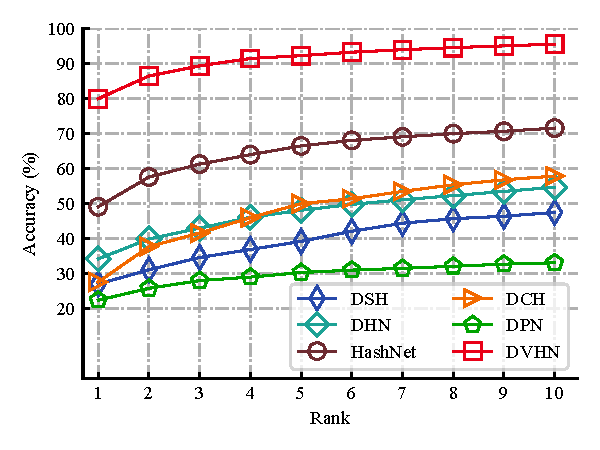
\includegraphics[height=5cm]{03/veri_256.pdf}
    \caption{在VeRi数据集下256位哈希码的各种模型的CMC结果}
  \end{subfigure}
  \hspace{1cm}
  \begin{subfigure}{0.45\textwidth}
    \centering
    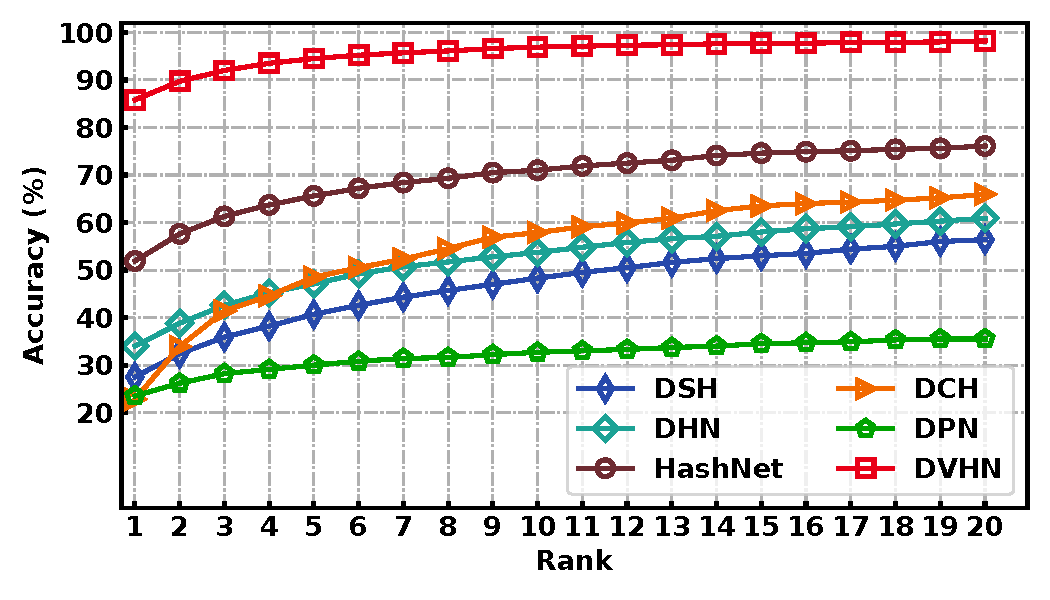
\includegraphics[height=5cm]{03/veri_512.pdf}
    \caption{在VeRi数据集下512位哈希码的各种模型的CMC结果}
  \end{subfigure}
  \begin{subfigure}{0.45\textwidth}
    \centering
    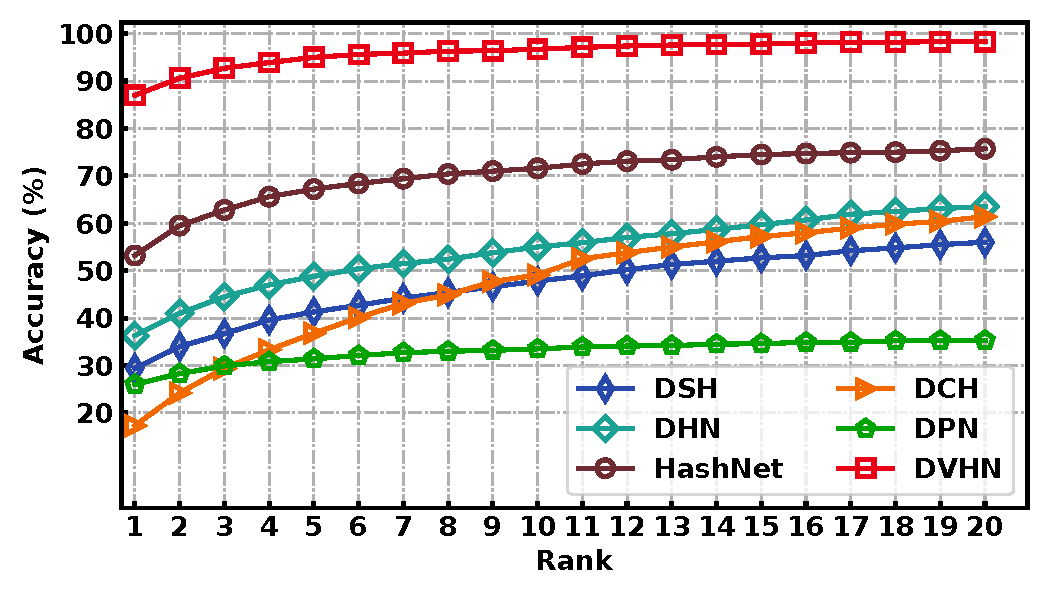
\includegraphics[height=5cm]{03/veri_1024.pdf}
    \caption{在VeRi数据集下1024位哈希码的各种模型的CMC结果}
  \end{subfigure}
  \hspace{1cm}
  \begin{subfigure}{0.45\textwidth}
    \centering
    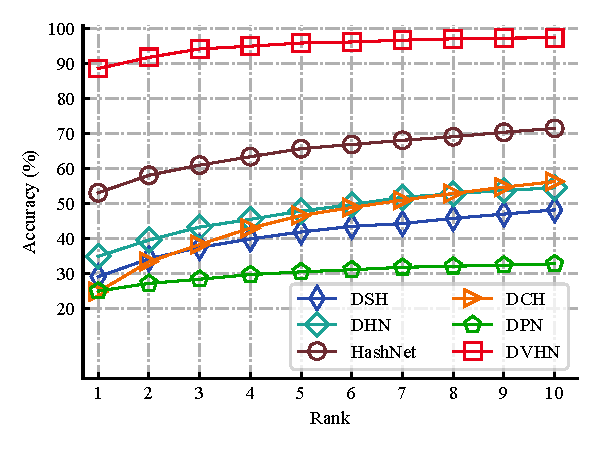
\includegraphics[height=5cm]{03/veri_2048.pdf}
    \caption{在VeRi数据集下2048位哈希码的各种模型的CMC结果}
  \end{subfigure}
  \begin{subfigure}{0.45\textwidth} .              
    \centering
    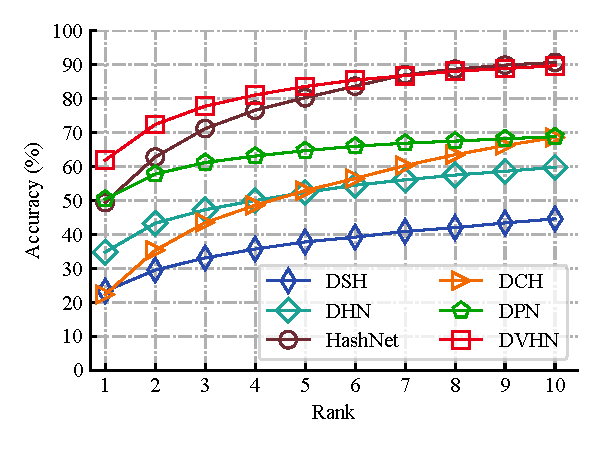
\includegraphics[height=5cm]{03/vid_256.pdf}
    \caption{在VehicleID (800)数据集下256位哈希码的各种模型的CMC结果}
  \end{subfigure}
  \hspace{1cm}
  \begin{subfigure}{0.45\textwidth}
    \centering
    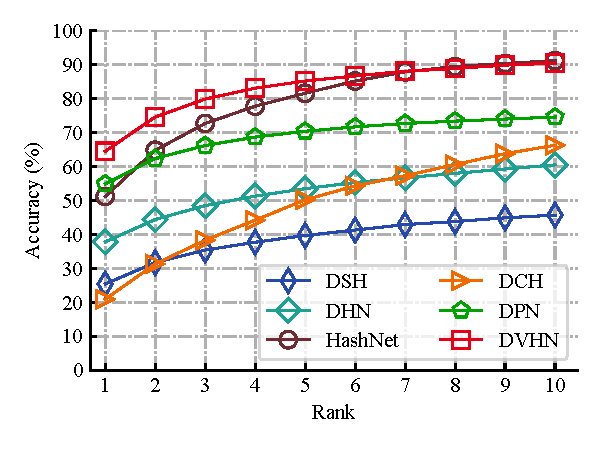
\includegraphics[height=5cm]{03/vid_512.pdf}
    \caption{在VehicleID (800)数据集下512位哈希码的各种模型的CMC结果}
  \end{subfigure}
\end{figure}
\begin{figure}[!htp]\ContinuedFloat
  \begin{subfigure}{0.45\textwidth}
    \centering
    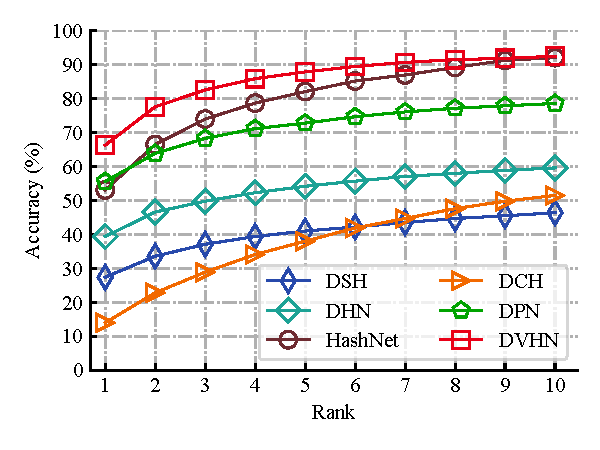
\includegraphics[height=5cm]{03/vid_1024.pdf}
    \caption{在VehicleID (800)数据集下1024位哈希码的各种模型的CMC结果}
  \end{subfigure}
  \hspace{1cm}
  \begin{subfigure}{0.45\textwidth}
    \centering
    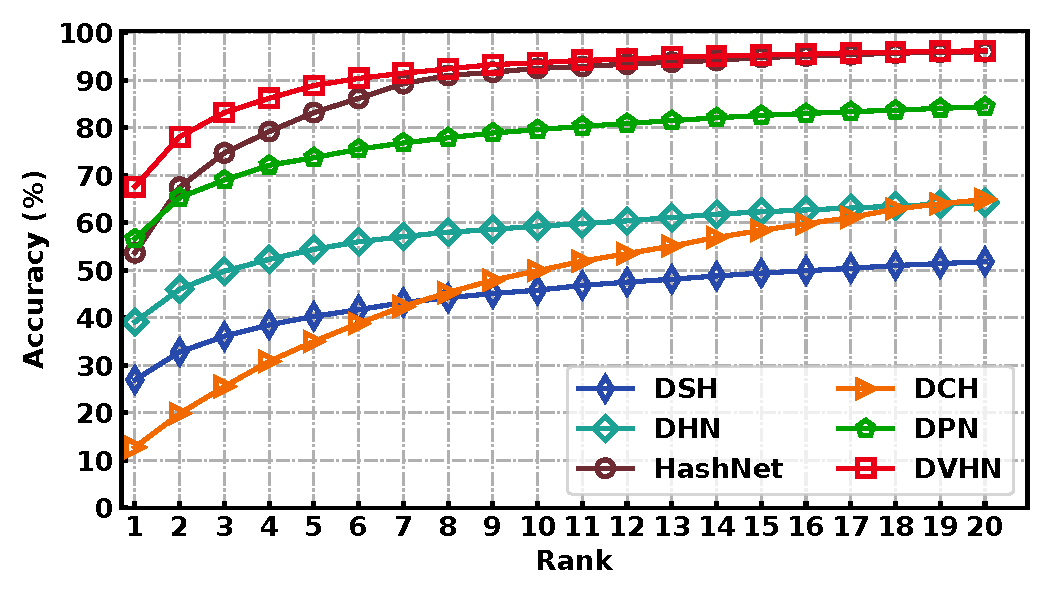
\includegraphics[height=5cm]{03/vid_2048.pdf}
    \caption{在VehicleID (800)数据集下2048位哈希码的各种模型的CMC结果}
  \end{subfigure}
  \begin{subfigure}{0.45\textwidth}
    \centering
    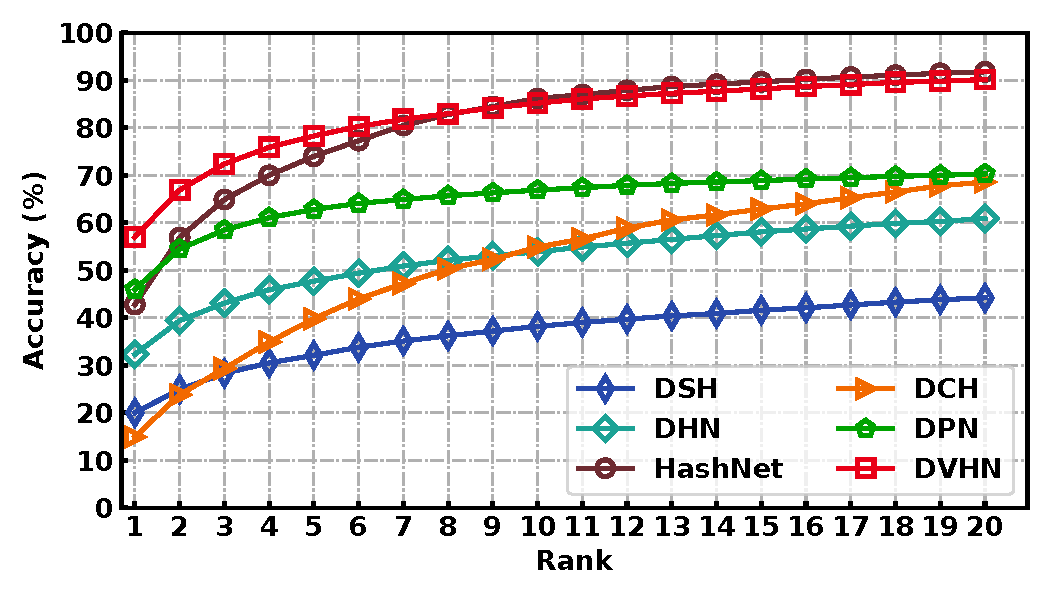
\includegraphics[height=5cm]{03/vid_1600_256.pdf}
    \caption{在VehicleID (1600)数据集下256位哈希码的各种模型的CMC结果}
  \end{subfigure}
  \hspace{1cm}
  \begin{subfigure}{0.45\textwidth}
    \centering
    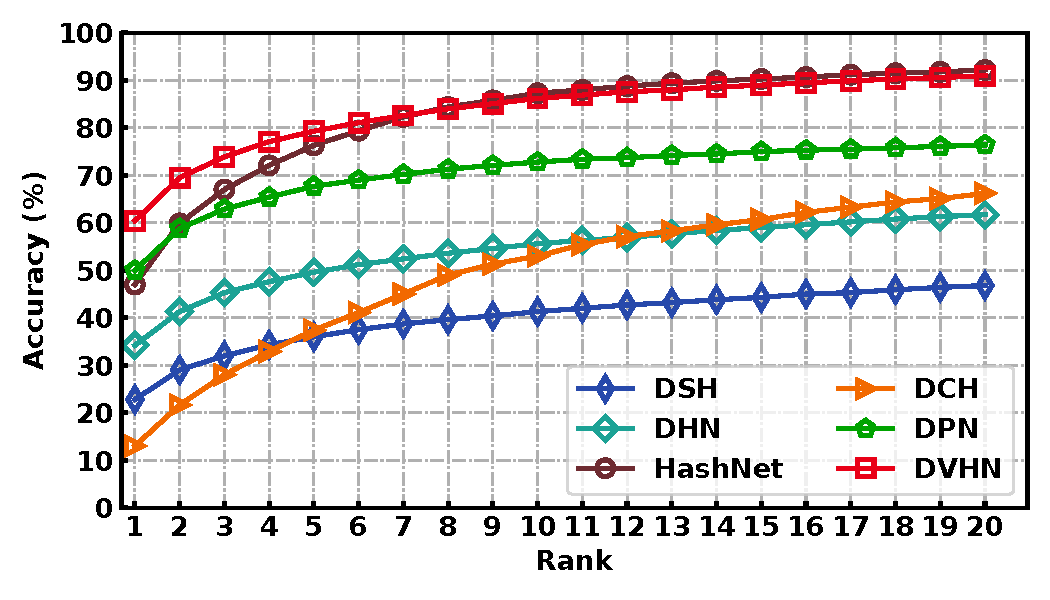
\includegraphics[height=5cm]{03/vid_1600_512.pdf}
    \caption{在VehicleID (1600)数据集下512位哈希码的各种模型的CMC结果}
  \end{subfigure}
  \begin{subfigure}{0.45\textwidth}
    \centering
    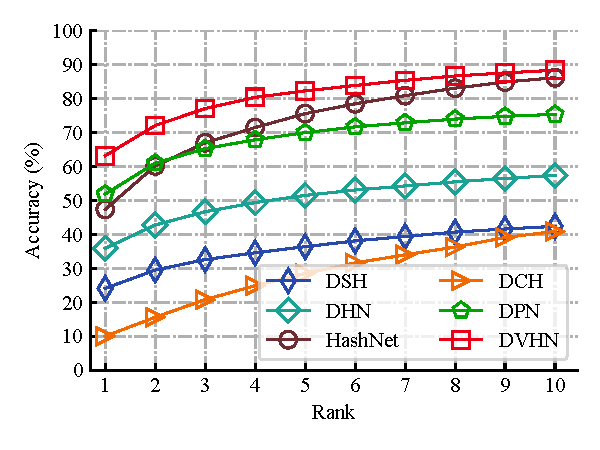
\includegraphics[height=5cm]{03/vid_1600_1024.pdf}
    \caption{在VehicleID (1600)数据集下1024位哈希码的各种模型的CMC结果}
  \end{subfigure}
  \hspace{1cm}
  \begin{subfigure}{0.45\textwidth}
    \centering
    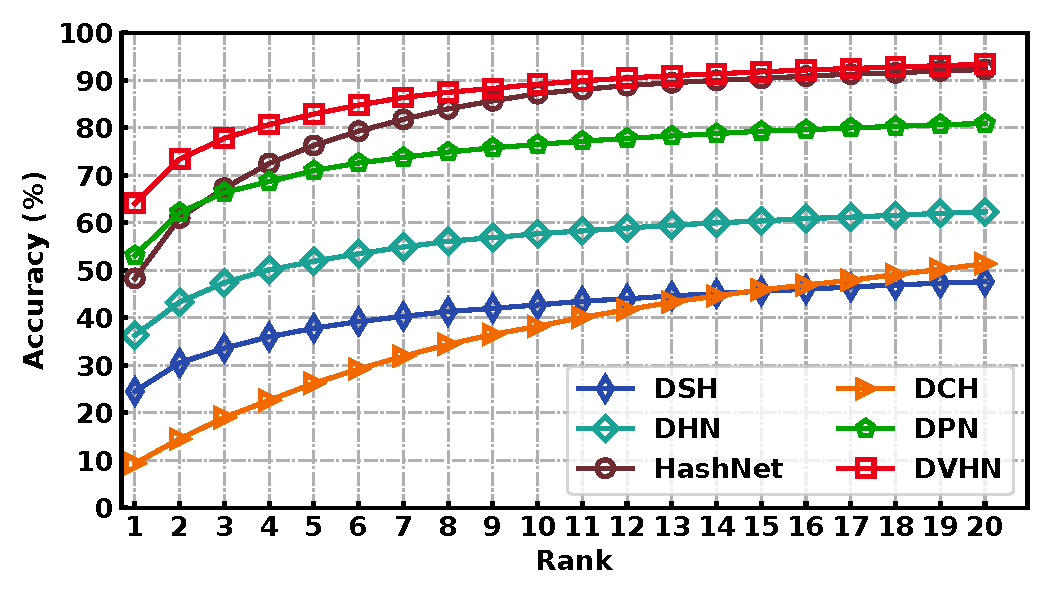
\includegraphics[height=5cm]{03/vid_1600_2048.pdf}
    \caption{在VehicleID (1600)数据集下2048位哈希码的各种模型的CMC结果}
  \end{subfigure}
 
  \bicaption[先进算法在两个数据集不同的哈希码长度下的性能比较结果]{各种先进算法在不同的哈希长度下在两个车辆检索公共数据集下的性能比较}{The vehicle re-identification results of different state-of-the-arts on two public benchmark datasets of varied hashing lengths.}
  \label{fig:vehashresults}
\end{figure}





另外, 我们也加入其他的最近的哈希方法进行细致的比较和分析, 包括~\textbf{DHN}~\cite{zhu2016deep}, \textbf{HashNet}~\cite{cao2017hashnet}, \textbf{DCH}~\cite{cao2018deep}, \textbf{DPN}~\cite{fan2020deep}。值得注意的是对于~\textbf{SH}, ~\textbf{ITQ},~\textbf{DCH}和~\textbf{DHN}我们采用作者开源的代码, 而对于其他的方法, 我们基于\textit{Pytorch}进行重新实现。我们首先对于所有的模型在生成哈希码为$2048$位的情况下进行分析。如表~\ref{table:vid800}, 表~\ref{table:vid1600}和表~\ref{table:veri}所示, 很明显, 传统的非深度学习的方法如~\textbf{SH}和~\textbf{ITQ}在两个数据集上都只能取得显著较低的性能。在哈希码长度为$2048$位是, 它们在\textbf{VeRi}数据集上分别取得$1.57\%$和$5.14\%$ \textbf{mAP}。 在\textbf{VehicleID (800)}和\textbf{VehicleID (1600)}上, 性能稍微有上升的趋势。具体来说, \textbf{SH}取得了$17.71 \%$ 和 $13.83 \%$ \textbf{mAP}而 \textbf{ITQ}分别达到了$26.26 \%$ 和 $22.23\%$。
\begin{figure}[!htp]
    \centering
    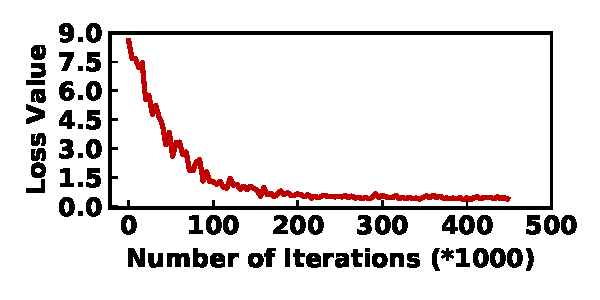
\includegraphics[height=3.5cm]{03/loss_256.pdf}
    \hspace{1cm}
    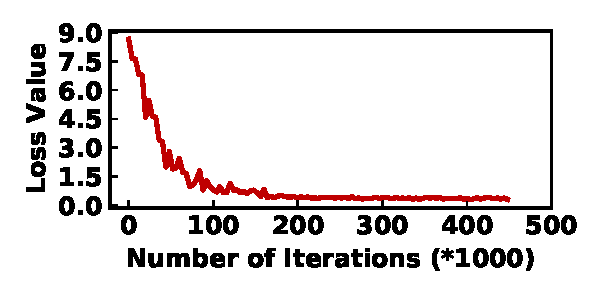
\includegraphics[height=3.5cm]{03/loss_512.pdf}
    \bicaption[\textbf{DVHN}在$256$和$512$哈希长度下的收敛图]{\textbf{DVHN}在$256$ (左)和$512$ (右)哈希长度下的收敛曲线}{The convergence curve of \textbf{DVHN} on 256 (left) and 512 (right) bits.}
    \label{fig:losscurve}
  \end{figure}

  \begin{figure}[!htp]
    \centering
    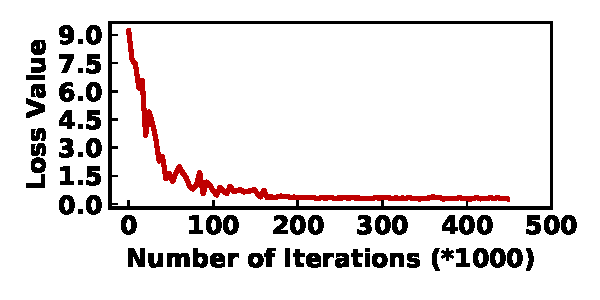
\includegraphics[height=3.5cm]{03/loss_1024.pdf}
    \hspace{1cm}
    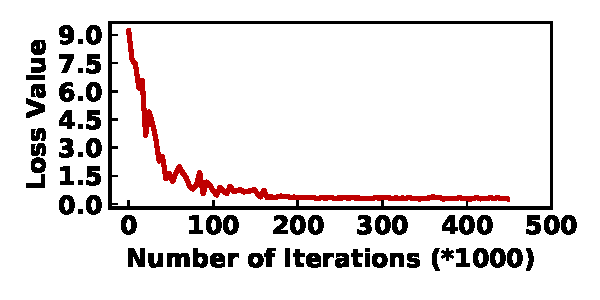
\includegraphics[height=3.5cm]{03/loss_2048.pdf}
    \bicaption[\textbf{DVHN}在$1024$和$2048$哈希长度下的收敛图]{\textbf{DVHN}在$1024$ (左)和$2048$ (右)哈希长度下的收敛曲线}{The convergence curve of \textbf{DVHN} on 1024 (left) and 2048 (right) bits.}
    \label{fig:losscurve1}
  \end{figure}


性能不优的主要原因是无监督的方法难以学习到具有判别力的特征, 从而导致了次优的哈希码。很明显, 监督的方法在两个数据集上在四种不同哈希码长度上都能取得更加优秀的结果。具体来说, ~\textbf{HashNet} 和 \textbf{DPN} 在\textbf{VehicleID (800)}上取得了优异的性能, 在 $2048$位的情况下分别取得 $66.61 \%$ 和 $64.65 \%$ \textbf{mAP}。对于其他哈希长度来说, 在\textbf{mAP} 这个指标下, 他们也是明显的赢家。 对于\textbf{VeRi}数据集, 两种算法的性能出现了明显的下降, 对于\textbf{HashNet}和\textbf{DPN} 分别取得 $29.30\%$ 和$13.58\%$。 性能的下降主要是由于\textbf{VeRi} 数据集是现实数据集, 有较大的背景遮挡, 视角变化等等带来的检索难度的提升。很明显, 本章提出的框架-\textbf{DVHN}-在所有的哈希长度以及在所有的测试数据集下都是优胜者。具体上, ~\textbf{DVHN}在$2048$位时, 在\textbf{VehicleID} 和\textbf{VeRi}上对于最先进的结果取得$11.05\%$和$35.46 \%$的\textbf{Rank-1}准确度提升。



对于$256$位的场景, 在两个数据集上, 我们获得了$11.54 \%$ 和 $30.93 \%$的提升。对于~\textbf{mAP}而言, 在$2048$位的哈希码长度场景下, 我们在\textbf{VehicleID (800)}, \textbf{VehicleID (1600)} 和 \textbf{VeRi}上, 我们分别取得了$76.82 \%$, $72.72 \%$ 和 $56.58 \%$。相比较次优的方法而言, 我们获得了$10.21 \%$, $11.30 \%$和$32.72\%$的性能提升。优越的性能可以证实我们的同时哈希和分类的设计可以使得模型学习到更具有判别性的特征, 生成更加紧凑的编码。\par 
我们额外提供了各个模型在不同的哈希长度情况下在~\textbf{VehicleID (800)}, ~\textbf{VehicleID (1600)}和~\textbf{VeRi}三种数据集下的\textbf{top-K} 准确度的结果(CMC 曲线), 如图~\ref{fig:vehashresults}所示。 \par
\textbf{VehicleID (800):} 如图~\ref{fig:vehashresults} (e,f,g,h)所示, 本章比较了~\textbf{DVHN}和其他深度哈希模型在不同的哈希长度下的 \textbf{top-K}准确度差异。值得注意的是, 由于无监督算法较低的性能表现, 我们并没有加入无监督的哈希算法进行比较。很明显可以发现, 在\textbf{Rank-1}到\textbf{Rank-5}, \textbf{DVHN}都取得了非常显著的性能提升。相比较~\textbf{DPN}而言 ~\textbf{DVHN}在$256, 512, 1024, 2048$ 哈希码长度的场景下分别取得取得了$11.52\%,~9.61\%,~10.75\% $和 $11.05\%$ 的性能提升。同时也能发现, ~\textbf{HashNet} 在\textbf{Rank-6}到\textbf{Rank-10}下也能取得比较优异的结果。然而在重识别任务中, 返回的匹配图片越靠前越满足检索需求。同时也能发现, 我们的模型在哈希码长度增加时能取得更加优异的结果, \textbf{mAP}从$71.61\%$提高到$76.81$。性能的提升主要归功于较长的哈希码可以保存更多的相似度信息。 \par


\begin{figure}[!htp]
    \centering
    \begin{subfigure}{0.45\textwidth}
      \centering
      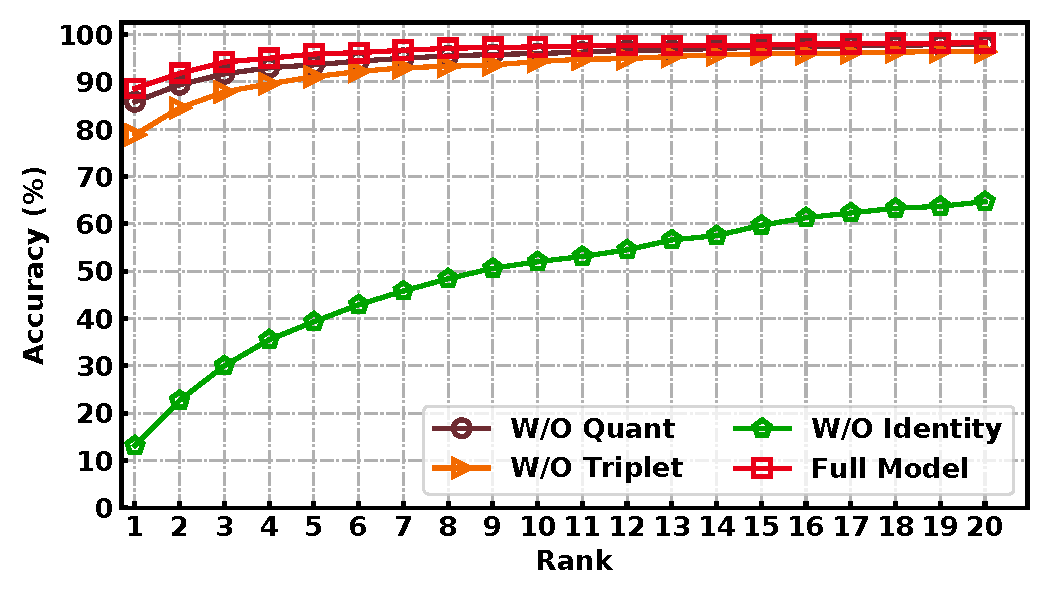
\includegraphics[height=5cm]{03/ablation_veri.pdf}
      \caption{不同的变种在\textbf{VeRi}数据集上的\textbf{CMC}曲线}
    \end{subfigure}
    \hspace{1cm}
    \begin{subfigure}{0.45\textwidth}
      \centering
      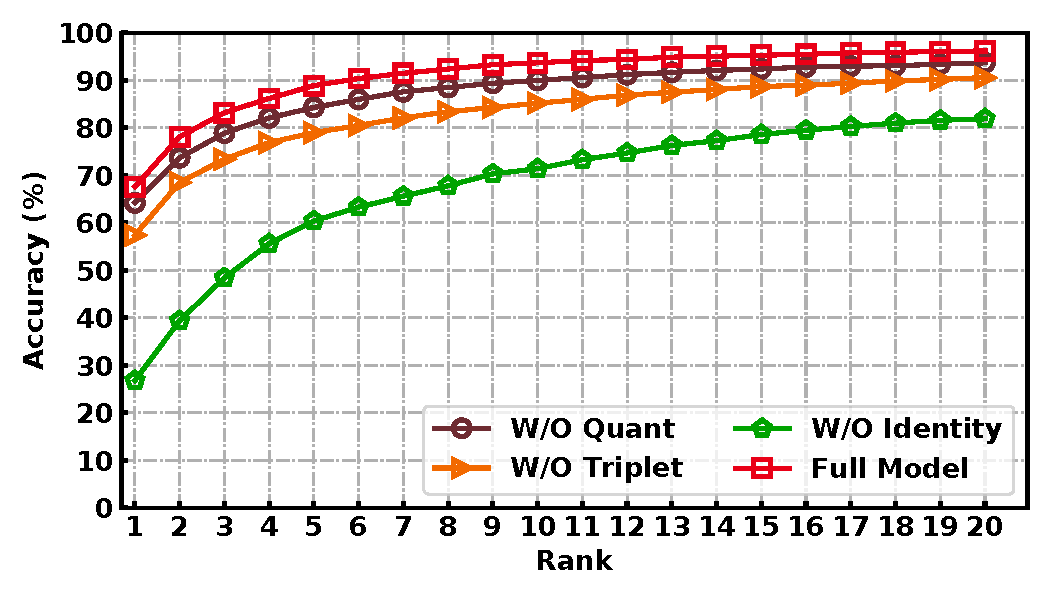
\includegraphics[height=5cm]{03/ablation_vid.pdf}
      \caption{不同的变种在\textbf{VehicleID}数据集上的\textbf{CMC}曲线}
    \end{subfigure}
    \bicaption[\textbf{DVHN}消融实验的\textbf{CMC}结果]{\textbf{DVHN}消融实验的在\textbf{VehicleID (800)} 和\textbf{VeRi}数据集上的\textbf{CMC}结果}{The ablation results on \textbf{VehicleID (800)} and \textbf{VeRI} of \textbf{DVHN}}
    \label{fig:ablationcmc}
  \end{figure}

\textbf{VehicleID (1600):}对于在这个场景下的性能表现, 如表~\ref{table:vid1600}, 图~\ref{fig:vehashresults} (i, j, k, l)所示, 在\textbf{CMC}和\textbf{mAP}上我们可以发现相似的趋势。\textbf{DVHN}在$256, 512, 1024$和$2048$位场景下可以取得$57.06\%, 60.41\%, 63.26\%,64.11\%$的\textbf{Rank-1}性能。对于\textbf{mAP}, \textbf{DVHN}可以在所有场景下均取得了大范围的性能提升。值得注意的是, 与\textbf{VehicleID (800)}的测试相比, 模型的性能有明显的下降。 例如, \textbf{Rank-1}准确度在哈希码长度为$256$位时, 下降了接近$5 \%$。这主要是由于数据库中照片增大导致的检索难度提升。 \par
\textbf{VeRi: }如表~\ref{table:veri}和图~\ref{fig:vehashresults} (a, b, c, d)所示, \textbf{DVHN}和其他所有比较的方法在所有的评估指标上都显示出了持续的优势。 如图~\ref{fig:vehashresults} (a, b, c, d)所示, ~\textbf{DVHN}大幅度领先\textbf{HashNet}。我们在$256,512,1024,2048$位哈希码的场景分别获得了$80.10\%, 85.81\%, 87.01\% $和 $88.62\%$的\textbf{Rank-1}准确度, 比~\textbf{HashNet}对应超出$30.93\%, 33.85\%, 33.73\%$ 和 $35.46\%$。对于~\textbf{mAP}而言, \textbf{DVHN}和其余比较的方法的性能差异更加显著。我们比第二优的方法在$2048$位的哈希码场景下超出了$32.77 \%$。明显, 在图~\ref{fig:vehashresults} (a, b, c, d)中, 代表~\textbf{DVHN}性能的红色曲线持续在其他曲线之上, 并且以大幅度领先。我们算法的优越性可以归功于我们的相似度保留的学习策略和离散哈希的模块的紧耦合的设计。

\begin{figure}[!htp]
    \centering
    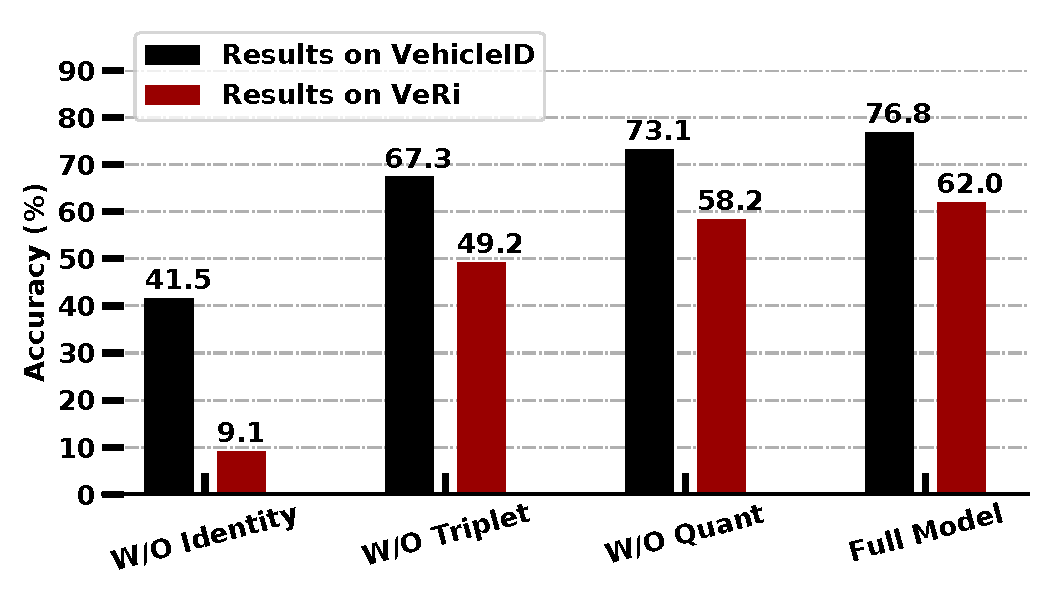
\includegraphics[width=15cm]{03/ablation_map.pdf} \\
    \bicaption[在\textbf{VehicleID (800)}和\textbf{VeRi}数据集上的消融实验\textbf{mAP}结果]
      {不同的变种在\textbf{VehicleID (800)}和\textbf{VeRi}数据集上的\textbf{mAP}}
      {The ablation results on \textbf{VehicleID (800)} and \textbf{VeRI} in terms of \textbf{mAP}}
   \label{fig:ablationmap}
\end{figure}

\subsection{经验性分析}
首先, 本章的模型在不同哈希长度下的收敛曲线如图~\ref{fig:losscurve}和图~\ref{fig:losscurve1}所示。\par
其次, 我们进行的详细的消融实验来证明\textbf{DVHN}框架中各个组成部分的效果。为了有效的评估身份损失函数$L_{Identity}$, 基于三元组的损失函数$L_{Triplet}$和我们设计的离散学习损失$L_{Quant}$, 我们设计了如下变种算法, 并且依次测试了他们在\textbf{VehicleID (800)}和\textbf{VeRi}数据集上的性能。
\begin{enumerate}
    \item \textbf{Full Model:} 一个包含了全部的部件的变种模型, 也就是完整版的\textbf{DVHN}。
    \item \textbf{W/O Triplet:} 缺少了基于三元组的相似度保留损失函数$L_{Triplet}$的模型。 
    \item  \textbf{W/O Identity:} 缺少了基于分类器的分类损失函数$L_{Identity}$的变种模型。
    \item \textbf{W/O Quant:} 缺少了离散哈希学习模块的变种模型。
\end{enumerate}
值得注意的是, 所有的消融实验是在哈希码为$2048$位的情况下进行。如图~\ref{fig:ablationcmc}和图~\ref{fig:ablationmap}所示, 

\begin{figure}[!htp]
    \centering
    \begin{subfigure}{\textwidth}
      \centering
      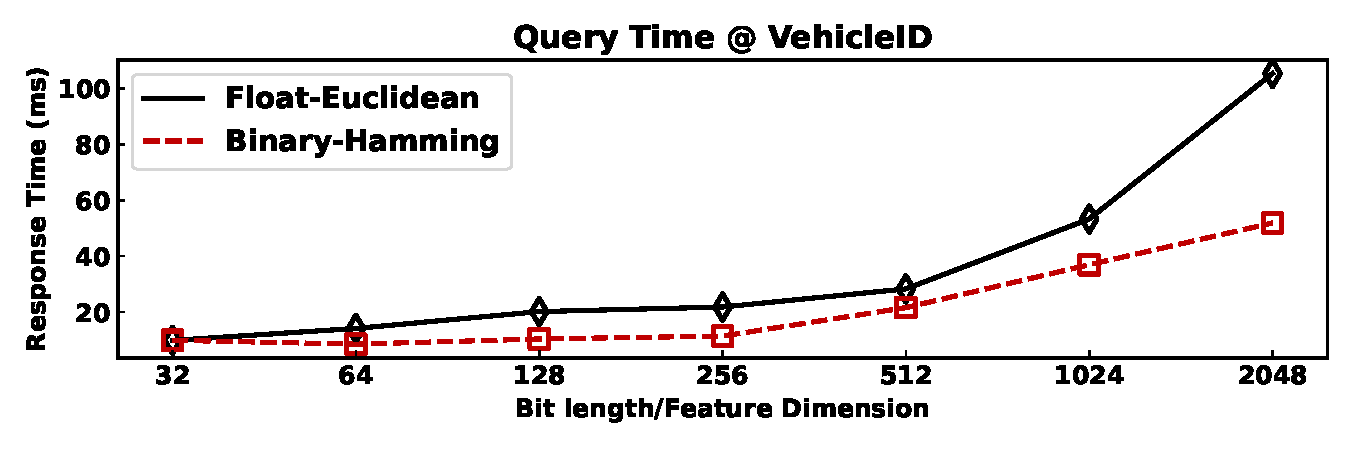
\includegraphics[height=4cm]{03/vehicle_query_speed.pdf}
      \caption{在\textbf{VehicleID}上的查询时间}
    \end{subfigure}
    \hspace{1cm}
    \begin{subfigure}{\textwidth}
      \centering
      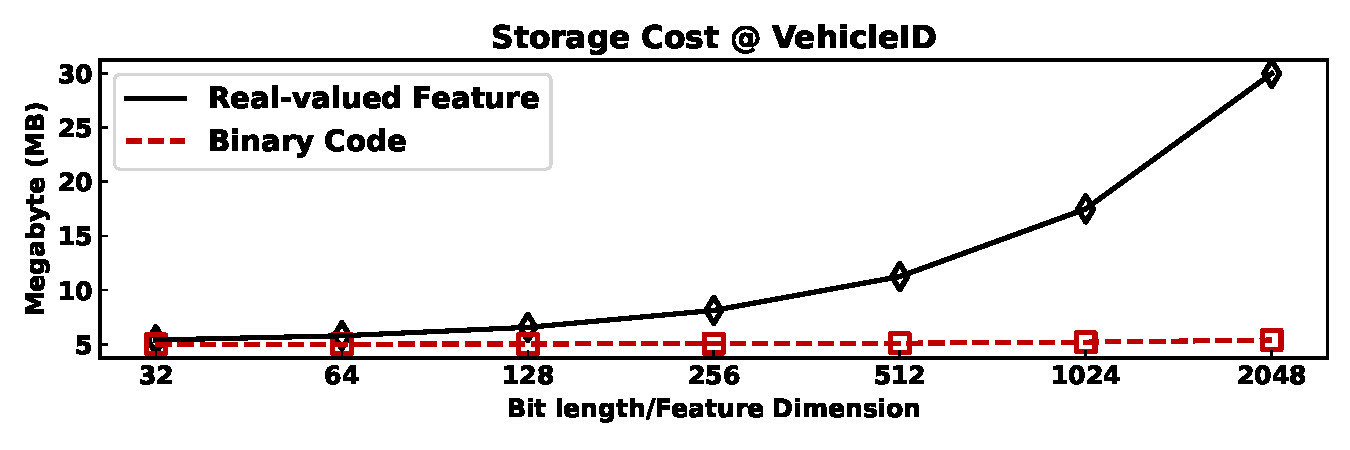
\includegraphics[height=4cm]{03/vehicle_storage.pdf}
      \caption{在\textbf{VehicleID}上的存储开销}
    \end{subfigure}
    \begin{subfigure}{\textwidth}
        \centering
        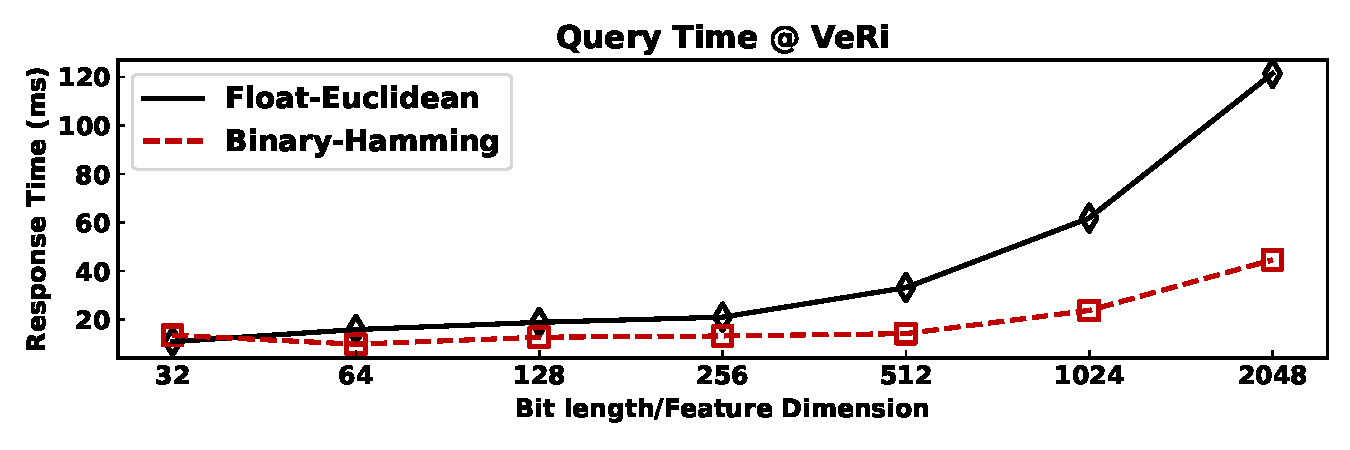
\includegraphics[height=4cm]{03/veri_query_speed.pdf}
        \caption{在\textbf{VeRi}上的查询时间}
      \end{subfigure}
      \begin{subfigure}{\textwidth}
        \centering
        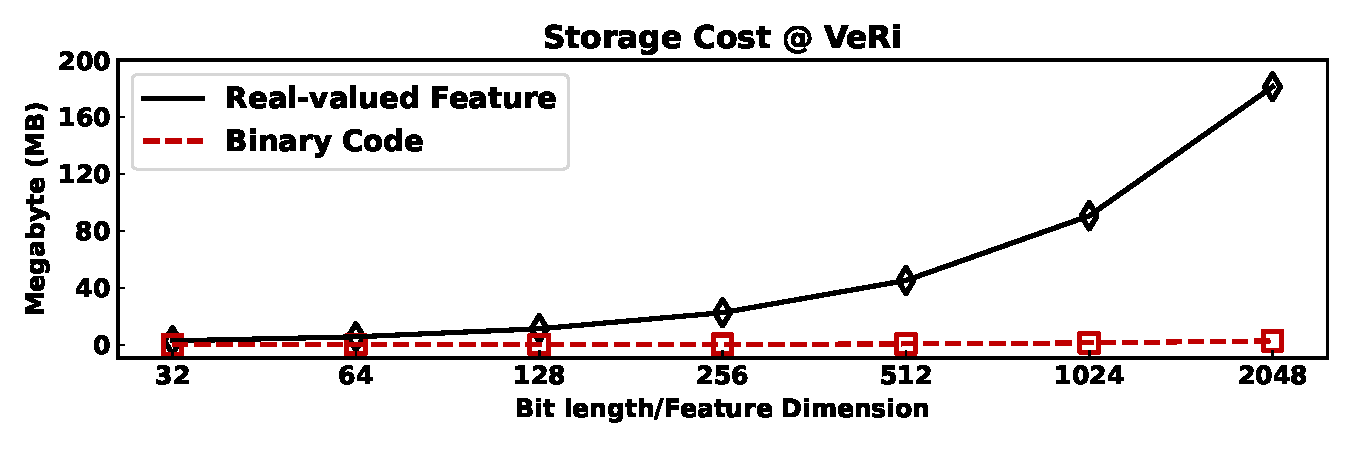
\includegraphics[height=4cm]{03/veri_storage.pdf}
        \caption{在\textbf{VeRi}上的存储开销}
      \end{subfigure}
    \bicaption[存储开销和查询时间的对比]{实值检索和基于哈希码的检索的存储开销和检索时间对比}{Comparison of the total query response time and storage cost of real-valued vectors and binary hash code}
    \label{fig:sttcost}
  \end{figure}
  当模型没有离散学习损失函数时, \textbf{Rank-1}准确度 和 \textbf{mAP} 在\textbf{VehicleID (800)}数据集上分别下降$3.46 \%$ 和 $3.50 \%$, 而在\textbf{VeRi}数据集上分别下降$2.80 \%$和$3.77 \%$。这证实了本章提出的离散学习模块在生成包含车辆信息的二进制编码的有效性。当模型失去$L_{Identity}$, 如图中的 \textbf{W/O Identity}所示, 模型的性能遭遇了显著的下降。具体来说, 在\textbf{VehicleID (800)}上, \textbf{Rank-1}准确度下降了$40.84 \%$而\textbf{mAP}则下降了$35.31 \%$。 在\textbf{VeRi}数据集上, 性能的下降更加的显著, \textbf{Rank-1}准确度下降了$75.11 \%$而\textbf{mAP}则下降了$52.84 \%$。性能的大幅度下降也证实了身份损失函数在学习强健并且有判别性特征方面的重要性。最后, 当我们观察没有了$L_{Triplet}$损失函数的橙色曲线\textbf{W/O Triplet}, 我们也可以观察到和\textbf{Full Model}对比的显著的性能下降。在\textbf{VehicleID (800)}上, \textbf{W/O Triplet}取得了$57.47 \%$的\textbf{Rank-1} 准确度和$67.32 \%$ 的\textbf{mAP}, 比\textbf{Full Model}分别下降了$10.19 \%$和$9.45 \%$。在\textbf{VeRi}数据集上, 我们也能观察到类似的趋势。\textbf{W/O Triplet}获得了$78.84$ \% \textbf{Rank-1}准确度和$49.23 \%$的\textbf{mAP}, 比\textbf{Full Model}降低了$9.78 \%$ 和 $12.79\%$。 模型性能的下降主要可以证明基于困难三元组的三元损失函数在解决车辆重识别问题的有效性, 特别是在类内变化有时候比类间变化更显著情况下。由此小节的消融实验可以证明各个部分的损失函数对于\textbf{DVHN}模型的整体性能都是不可缺少的。 
  
\begin{figure}[!htp]
    \centering
    \includegraphics[width=15.5cm]{03/256_retrieved_results.pdf} \\
    \bicaption[256位的\textbf{DVHN}框架的检索结果可视化]
      {256位的\textbf{DVHN}框架在\textbf{VehicleID (800)}数据集上的的前十检索结果可视化}
      {The Visualization of the Top 10 Retrieved Results of \textbf{DVHN} Framework on 256 Hashing Bit}
   \label{fig:retrieval256}
\end{figure}
\subsection{检索效率比较}
车辆重识别 (Vehicle ReID)系统的检索时间开销一般分为两个部分: ``特征提取的时间开销''和``向量距离计算的时间开销''。如Chen等人~\cite{chen2020deep}指出, 特征提取的时间开销其实绝大部分和使用的主干神经网络相关, 因此, 我们固定使用同样的神经网络模型。 在本小节的比较中, 我们主要关注比较我们方法的大规模的距离计算的时间开销和基于实值向量的大规模计算的开销。 同时, 我们也和基于实值向量的方法比较我们基于二进制汉明哈希码的存储开销。\par
如图~\ref{fig:sttcost} 所示, 我们展示了在\textbf{VehicleID (1600)}和\textbf{VeRi}上的检索效率对比。 其中\textbf{VehicleID (1600)}包含$11,777$张查询图片, $1,600$张数据库照片, 而 \textbf{VeRi}包含了$1,678$张查询图片和$11,579$张数据库照片。在图~\ref{fig:sttcost}中a和c, ``Float-Euclidean''表示基于实值向量的车辆重识别方法在数据集上进行大规模欧式距离计算的时间开销。而``Binary-Hamming''表示基于二进制哈希码的车辆重识别方法在数据集上进行大规模汉明距离计算的时间开销。对于图(c)和图(d), 其展示了两种不同的方法在两个数据集上不同的向量长度的存储开销。 非常明显可以看出基于二进制哈希码的方法可以大量降低存储的开销以及提高检索的速度。
\begin{figure}[!htp]
    \centering
    \includegraphics[width=15.5cm]{03/512_retrieved_results.pdf} \\
    \bicaption[512位的\textbf{DVHN}框架的检索结果可视化]
      {512位的\textbf{DVHN}框架在\textbf{VehicleID (800)}数据集上的的前十检索结果可视化}
      {The Visualization of the Top 10 Retrieved Results of \textbf{DVHN} Framework on 512 Hashing Bit}
   \label{fig:retrieval512}
\end{figure}
\begin{figure}[!htp]
    \centering
    \includegraphics[width=15.5cm]{03/1024_retrieved_results.pdf} \\
    \bicaption[256位的\textbf{DVHN}框架的检索结果可视化]
      {1024的\textbf{DVHN}框架在\textbf{VehicleID (800)}数据集上的的前十检索结果可视化}
      {The Visualization of the Top 10 Retrieved Results of \textbf{DVHN} Framework on 1024 Hashing Bit}
   \label{fig:retrieval1024}
\end{figure}
\begin{figure}[!htp]
    \centering
    \includegraphics[width=15.5cm]{03/2048_retrieved_results.pdf} \\
    \bicaption[256位的\textbf{DVHN}框架的检索结果可视化]
      {2048位的\textbf{DVHN}框架在\textbf{VehicleID (800)}数据集上的的前十检索结果可视化}
      {The Visualization of the Top 10 Retrieved Results of \textbf{DVHN} Framework on 2048Hashing Bit}
   \label{fig:retrieval2048}
\end{figure}
\subsection{车辆检索结果的定性分析}
在图~\ref{fig:retrieval256}, 图~\ref{fig:retrieval512}, 图~\ref{fig:retrieval1024}和图~\ref{fig:retrieval2048}中, 我们可视化\textbf{DVHN}再不同的哈希码长度的场景在\textbf{VeRi}数据集上的检索结果。为了展示检索的有效性, 我们将原先的数据库集当成查询集, 将查询集当作被检索的数据库集, 这样的话每一张查询的图片在数据库中有多个对应的图片。在上述的可视化图中, 为了方便对比性能, 我们采用同一张查询的图片在$256$, $512$, $1024$, $2048$四个长度的哈希码场景下进行检索。图的右侧可视化了对于查询图片生成的前十张检索图片。蓝色框圈出来的图片代表它和查询图片是属于同一辆车。通常来说, 对于一个重识别的模型, 我们希望在检索返回的图片中属于同一辆车的图片尽量靠前。在四张可视化图中也可以看出来, $2048$位的哈希检索模型有更加好的检索效果。
\subsection{总结}
本章基于深度哈希学习提出了第一个进行高效大规模车辆重识别的框架-\textbf{DVHN}。受深度哈希采用二进制哈希码来进行高效的检索的启发, 我们进行第一个引入二进制哈希算法进行解决大规模车辆重识别问题, 和传统基于实值的检索方法相比, 极大的的降低了存储的开销以及提高了检索的速度。具体来说, 对于相似度保持的度量学习, 本章采取了一个三元损失函数以及一个设计了在线困难三元组生成模块。同时, 我们额外增加了一个基于分类损失的身份损失函数来学习更强健和有判别性的特征表示。 对于二进制码学习, 我们基于二进制码应该尽量保留图像的类别信息的假设, 提出了一个离散哈希学习方法。 为了解决由于生成二进制码使用\textit{sign}函数带来的梯度消失的难题, 我们提出一个交叉优化的方法来优化整个框架。我们在标准的大规模车辆数据集上进行了大规模广泛的实验。 实验结果表明本章提出的框架~\textbf{DVHN}可以生成有效的二进制哈希码来进行大规模的车辆检索, 并且相比较当前的其他先进的深度哈希方法, 我们的方法可以大幅度的提升检索的精度。

